\documentclass[english]{AMmasterArbeit}
\def\mainpath{.}
\def\tikzpath{./fig/tikz}
\def\studypath{../studies}
%\usepackage[utf8]{inputenc}
%\usepackage{textcomp}

%AMlatex template stuff
\usepackage{booktabs}
\usepackage{pdflscape}
\usepackage{longtable}
\usepackage{footnote}
\usepackage{import}
\usepackage{subcaption}
\usepackage{mycommands}


\usepackage{amsmath}
\usepackage{amsfonts}
\usepackage{amssymb}

\usepackage{graphicx}
\usepackage{pgfplots}
\usepackage{pgfplotstable}

%\usepackage{fancyhdr}
%\usepackage{graphicx}
%\usepackage{epstopdf}

\usepackage{struktex}

\usepackage{kbordermatrix}
\usepackage{blkarray}% http://ctan.org/pkg/blkarray

\usepackage[font={small,it}]{caption}

\usepackage[outline]{contour}

%\usepackage[subpreambles=true]{standalone}
%\usepackage{import}

%\usepackage{hyperref}
%\hypersetup{
%    colorlinks=true,
%    linkcolor=blue,
%    urlcolor=red,
%    linktoc=all
%}

%\usepackage[left=1.5cm,right=1.5cm,top=2cm,bottom=2cm]{geometry}

\extrafloats{200}




\definecolor{list1_1}{RGB}{0,101,189}
\definecolor{list1_2}{RGB}{156,157,159}
\definecolor{list1_3}{RGB}{162,173,0}
\definecolor{list1_4}{RGB}{227,114,34} 
\definecolor{list1_5}{RGB}{152,198,234}


%\definecolor{list1_1}{RGB}{246,81,29}
%\definecolor{list1_2}{RGB}{255,180,0}
%\definecolor{list1_3}{RGB}{0,166,237}
%\definecolor{list1_4}{RGB}{127,184,0}
%\definecolor{list1_5}{RGB}{13,44,84}


\pgfplotscreateplotcyclelist{markerlist}{
list1_1, thick, solid, mark=*\\%
list1_2, thick, solid, mark=asterisk\\%
list1_3, thick, solid, mark=diamond*\\%
list1_4, thick, solid, mark=triangle\\%
list1_5, thick, solid, mark=square\\%
}

\pgfplotscreateplotcyclelist{linelist}{
list1_1, solid\\%
list1_2, solid\\%
list1_3, solid\\%
list1_4, solid\\%
list1_5, solid\\%
}

\definecolor{lightgrey}{RGB}{200,200,200}
\definecolor{nassitextcolor}{RGB}{0,0,200}

\usetikzlibrary{pgfplots.groupplots}
\usetikzlibrary{patterns, shapes}

\usepgfplotslibrary{groupplots}

\pgfplotscreateplotcyclelist{convergelist}{
s2_1, thick, solid, mark=*\\%
s2_2, thick, solid, mark=square\\%
s2_3, thick, solid, mark=diamond*\\%
s2_4, thick, solid, mark=triangle\\%
s2_5, thick, solid, mark=asterisk\\%
}

\pgfplotscreateplotcyclelist{elelist}{
s2_1, solid\\%
s2_2, solid\\%
s2_3, solid\\%
s2_4, solid\\%
s2_5, solid\\%
}

\renewcommand{\vec}[1]{\boldsymbol{#1}}
%\renewcommand{\mat}[1]{\boldsymbol{#1}}

\newcommand{\derivtime}[1]{\dot{#1}}           % time derivative
\newcommand{\dderivtime}[1]{\ddot{#1}}         % double time derivative

%\renewcommand{\dd}{\mathrm{d}}                    % differential d
\newcommand{\pd}{\partial}                      % partial differentiation d

\newcommand{\dvec}[1]{\boldsymbol{ \mathsf{#1} } }         % for vectors
\newcommand{\dmat}[1]{\boldsymbol{\mathsf{#1}}}           % for matrices
\newcommand{\tensor}[1]{\boldsymbol{\mathcal{#1}}}
\newcommand{\Bd}[2]{ (#1,#2)_{D^k} }           % bilienarfor over domian
\newcommand{\Bb}[2]{ (#1,#2)_{\partial D^k} }           % bilienarfor over boundary
\newcommand{\0}{\textcolor{lightgrey}{0}}
%
\newcommand{\domainone}{\Omega_1}
\newcommand{\domaintwo}{\Omega_2}
\newcommand{\ifaceone}{\Gamma_1}
\newcommand{\ifacetwo}{\Gamma_2}

\newcommand{\stiffmat}{\dmat{K}}

\newcommand{\condnum}{\mathcal{K}}
\newcommand{\myorder}[1]{\mathcal{O}\left(#1\right)}

\newcommand{\sfn}{N}

\newcommand{\disp}{u}
\newcommand{\dispvec}{\dvec{\disp}}

\newcommand{\lag}{\lambda}
\newcommand{\lagvec}{\dvec{\lag}}

%natural coarse space lambda
\newcommand{\lagn}{\lambda_N}
\newcommand{\lagnvec}{\dvec{\lagn}}

%Coarse space lambda
\newcommand{\lagc}{\lambda_C}
\newcommand{\lagcvec}{\dvec{\lagc}}

%FETI subspace space lambda
\newcommand{\lagf}{\lambda_F}
\newcommand{\lagfvec}{\dvec{\lagf}}


\newcommand{\rmode}{\alpha}
\newcommand{\rmodevec}{\dvec{\rmode}}

\newcommand{\force}{f}
\newcommand{\forcevec}{\dvec{\force}}

\newcommand{\ifacedisp}{d}
\newcommand{\ifacedispvec}{\dvec{\ifacedisp}}

\newcommand{\res}{r}
\newcommand{\resvec}{\dvec{\res}}

\newcommand{\traceop}{\dmat{t}}
\newcommand{\asmop}{\dmat{B}}
\newcommand{\nullspacemat}{\dmat{R}}
\newcommand{\locschur}{\dmat{S}}
\newcommand{\asmlocschur}{\asmids{\dmat{S}}}
\newcommand{\locdualschur}{\dmat{F}}

\newcommand{\precond}{\dmat{F}}


\newcommand{\rmodespace}{\dmat{G}}
\newcommand{\scalemat}{\dmat{A}}

\newcommand{\cspace}{\dmat{C}}
\newcommand{\projn}{\dmat{P}}
\newcommand{\projc}{\dmat{P}_c}

\newcommand{\totalgap}{\dvec{\Delta}}

%feti-general
\newcommand{\evec}{\dvec{e}}

%feti-2
\newcommand{\sdirnspacecspace}{\dvec{q}}
\newcommand{\sdirnspace}{\dvec{w}} %search direction
\newcommand{\sdirfspace}{\dvec{z}}

%feti-s
\newcommand{\sdirnspacemat}{\dmat{W}}
\newcommand{\Zmat}{\dmat{Z}}
\newcommand{\sdirfspacemat}{\dmat{Z}}
\newcommand{\Deltamat}{\dmat{\Delta}}
\newcommand{\sdirnspacecspaceblock}{\dmat{Q}}

\newcommand{\eyemat}{\dmat{I}}

\newcommand{\idone}[1]{{#1}^{(1)} }
\newcommand{\idtwo}[1]{{#1}^{(2)} }
\newcommand{\ids}[1]  {{#1}^{(s)} }
\newcommand{\asmids}[1]  {{#1}^{[s]} }
\newcommand{\inv}[1]  {{#1}^{-1} }
\newcommand{\pinv}[1] {{#1}^{+} }
\newcommand{\tp}[1]   {{#1}^{T} }
%\newcommand{\scaled}[1]{\tilde{#1}}
\newcommand{\scaled}[1]{#1}




%commands for chapter finite element method
\newcommand{\bodyforce}[1]{\dvec{\hat{b}}}
\newcommand{\stress}{\dvec{\sigma}}
\newcommand{\strain}{\dvec{\epsilon}}
\newcommand{\traction}{\dvec{t}}
%\newcommand{\pd}[1]{\partial}



%\newcommand{\nassitext}[1]{\textit{\textcolor{nassitextcolor}{#1}}}
\newcommand{\nassitext}[2]{\makebox[#1\textwidth]{\textit{\textcolor{nassitextcolor}{\small #2}}\hfill}}

\newcommand{\nassitextbold}[2]{\makebox[#1\textwidth]{\textbf{\textit{\textcolor{nassitextcolor}{\small #2}}}\hfill}}

\newcommand{\nassitexttwolines}[3]{\nassitext{#1}{#2}\hspace*{\hsize}\linebreak \nassitext{\df2}{#3}}

\usepackage{soul}
\definecolor{hlcolor}{RGB}{230,230,230}
\setulcolor{red}
%\newcommand{\hlchange}[1]{\colorbox{hlcolor}{$#1$}}
%\newcommand{\hlchange}[1]{\ul{$\displaystyle#1$}}
%\usepackage{xcolor}
\newsavebox\MBox
\newcommand\hlchange[2][red]{{\sbox\MBox{$#2$}%
  \rlap{\usebox\MBox}\color{#1}\rule[-1.7\dp\MBox]{\wd\MBox}{1.0pt}}}



\newcommand*\MyScale{1}
\newcommand*\Scale[1][1]{\renewcommand*\MyScale{#1}}
\tikzset{%
  every picture/.style={%
    scale=\MyScale,
  }
}


%\renewcommand\thesection{\roman{section}}
%\renewcommand\thesubsection{\thesection.\roman{subsection}}
%\renewcommand\thesubsubsection{\thesection.\thesubsection.\roman{subsection}}

\author{\text{Lukas Scheucher, B.Sc.}}
\title{Development and Analysis of Multi Preconditioned FETI Methods}
\date{19.\,09.~2016}
\supervisor{Michael Leistner, Dipl. Ing. \newline Prof. Dr. Daniel J. Rixen}
\addbibresource{literature.bib}
%\usepackage{hyperref}
%\usepackage{cite}
%\bibliography{literature.bib}

\usepackage{blindtext}
%\usepackage{showframe}

\usepackage[subpreambles=false]{standalone}

\usetikzlibrary{positioning}
\usepackage{pgfplots}
\usepackage{pgfplotstable}
\usepgfplotslibrary{groupplots}

%\usepackage{showlabels}
%\usepackage[subsection]{placeins}



%%%%%%%%%%%%%%%%%%%%%%%%%%%%%%%%%%%%%%%%%%%%%%%%%%
%\includeonly{cha_feti-solvers}
%%%%%%%%%%%%%%%%%%%%%%%%%%%%%%%%%%%%%%%%%%%%%%%%%%%%%

%\setlength{\footskip}{10mm}
%\footskip=1pt

\begin{document}
\frontmatter
\maketitle
%%%%\chapter*{Danksagung}


%\markright{Formelzeichenverzeichnis}
%\markboth{Formelzeichenverzeichnis}{Formelzeichenverzeichnis} 


Mein besonderer Dank gilt Dipl.-Ing. Johannes Mayet für die Betreuung meiner Master's Thesis
und die Vergabe der interessanten Aufgabenstellung. 
Für  seine geduldigen Erläuterungen bei Rückfragen zur zugrunde liegenden Theorie,
seine motivierenden  Ratschläge 
und die freundliche, hilfreiche und umfangreiche 
Unterstützung während der gesamten Bearbeitungszeit
bedanke ich mich sehr herzlich.
\PrintTablesAndListsOfContents
\section*{Nomenclature}\label{sec:nomenclature}
\subsection*{Representation of scalars. tensors and other quantities}
\begin{tabular}{l l}
$q,Q$      &Scalar quantity  \\
$\vec{q}$  &Continuous vectorial quantity  \\
$\mat{Q}$  &Continuous matrix quantity \\
$\dvec{q}$ &Discrete vectorial quantity  \\
$\dmat{Q}$ &Discrete matrix quantity \\
\end{tabular}


\subsection*{Operators and symbols}
\begin{tabular}{l l}
$\tp{(\cdot)}$   &Transpose of a tensor  \\
$\inv{(\cdot)}$  &Inverse of a tensor or mapping  \\
$\pinv{(\cdot)}$ &Pseudoinverse of a tensor or mapping  \\
$\derivtime{(\cdot)},\dderivtime{(\cdot)}$ &First and second time derivative at a fixed reference position  \\
%$\hat{(\cdot)}$ &prescribed quantity  \\
%$(\cdot,\cdot)_\mathrm {\lebesgue}$ &$\lebesgue$-inner product in $\Omega$  \\
%$(\cdot,\cdot)_\mathrm {\sobolev}$ &$\sobolev$-inner product in $\Omega$  \\
$\mathrm det$ &Determinant  \\
$\mathrm div$ &Spatial divergence operator  \\
$\pd$ &Virtual quantity  \\
\end{tabular}


\subsection*{FE space discretization}
\begin{tabular}{l l}
$\mathrm{nele}$ &Number of elements \\
$\mathrm {nnod}$ &Number of nodes \\
$\mathrm {ndim}$ &Number of spatial dimensions \\
$\mathrm {ndof}$ &Number of degrees of freedom \\
$\sfn_\mathrm k$ &FE shape function of node k \\
%$\sfdual_\mathrm k$ &FE dual shape function of node k \\
$\vec{\xi}$ &Position in FE parameter space \\
$\vec{\d X}$ &Discrete nodal positions in reference configuration \\
$\vec{\d x}$ &Discrete nodal positions in current configuration \\
$\vec{\d D}$ &Discrete nodal displacements in reference configuration \\
$\vec{\d d}$ &Discrete nodal displacements in current configuration \\
$\vec{\d X}$ &Discrete nodal positions in reference configuration \\
$h$ &Characteristic element size \\
$p$ &Polynomial degree of finite element interpolation \\
%$\mmat$ &Mass matrix \\
%$\dampmat$ &Damping matrix \\
%$\vec{\d f}$ &Discrete force vector \\
%$\stiff_\mathrm 0$ &Initial tangent stiffnes matrix
\end{tabular}
%

\subsection*{Domain decomposition}
\begin{tabular}{l l}
$\Omega_s$   &Domain with index $s$ \\
$\Gamma_s$   &Interface with index $s$\\
$\ids{(\cdot)}$      &Quantity related to domain $s$ \\
\end{tabular}

\subsection*{FETI-Method}
\subsubsection*{General}
\begin{tabular}{l l}
$\ids{(\cdot)}$   &substructure local quantity  \\
$\asmids{(\cdot)}$   &assembled substructure local quantity  \\
$\lag$      &Lagrange multiplier (can be interpreted as interface force)\\
$\lagvec$   &Vector of Lagrange multipliers\\
$\lagnvec$   &Vector of Lagrange multipliers in the natural subspace\\
$\lagcvec$   &Vector of Lagrange multipliers in the auxiliary(coarse) space\\
$\lagfvec$   &Vector of Lagrange multipliers in the conjugate gradient iteration space\\
$\rmodevec$ &Generalized coordinates of rigid body modes\\
$\force$    &External force (one component)\\
$\forcevec$ &Vector of external forces (dof-based)\\
%$\ifacedisp$ & Interface displacement solution\\
$\ifacedispvec$ &Interface displacements\\
$\res$      &Displacement gap(residuum)\\
$\resvec$   &Vector of residua\\
$\traceop$  &Trace operator\eqref{eq:asmop_and_traceop_example}\\
$\asmop$    &Boolean assembly operator \eqref{eq:asmop_and_traceop_example}\\
$\nullspacemat$ &Rigid body modes\\
$\locschur$ &Local Schur complement \eqref{eq:locschur}\\
$\locdualschur$ &Local Dual Schur complement\\
$\rmodespace$     &Constraint matrix\\
$\scalemat$ &Scaling matrix\\
$\cspace$   & Auxiliary Coarse space\\
$\projn$    &Projector to natural coarse space\\
$\projc$    &Projector to auxiliary coarse space\\
$\condnum$  &Condition number\\
\end{tabular}
\subsubsection*{FETI-2}
\begin{tabular}{l l}
$\sdirnspacecspace$ & Search direction in natural subspace\\
%$\wvec$ & TODO\\
$\sdirfspace$ & Search direction in conjugate gradient iteration space\\
\end{tabular}
\subsubsection*{FETI-S}
\begin{tabular}{l l}
$\sdirnspacecspaceblock$ & Block of search directions in natural subspace\\
$\sdirnspacemat$ & Search directions in natural subspace\\
$\Zmat$ & Block of search directions in conjugate gradient iteration space\\
%$\Deltamat$ & TODO
\end{tabular}

\subsubsection*{FETI-AS}
\begin{tabular}{l l}
$\tau$ & Adaptivity criterion\\
$t_i^s$ & Convergence Indicator\\
$\rho$ & Contraction factor\\
\end{tabular}

%\subsubsection*{FETI-B}
%\begin{tabular}{l l}
%a & a\\
%a & a\\
%\end{tabular}
%\subsubsection*{FETI-G}
%\begin{tabular}{l l}
%a & a\\
%a & a\\
%\end{tabular}
%\subsubsection*{FETI-A}
%\begin{tabular}{l l}
%a & a\\
%a & a\\
%\end{tabular}

\subsection*{Abbreviations}
\begin{tabular}{l l}
\textbf{DD}  &Domain Decomposition  \\
\textbf{BDD}  &Balanced Domain Decomposition  \\
\textbf{FETI}  &Finite Element Tearing and Interconnecting\\
\textbf{FETI-1} &One-level FETI algorithm\\
\textbf{FETI-2} &Two-level FETI algorithm\\
\textbf{FETI-S} &Simultaneous FETI algorithm\\
\textbf{FETI-B} &Block FETI algorithm\\
\textbf{FETI-AS} &Adaptive Simultaneous FETI algorithm\\
\textbf{FETI-FAS} &Fast Adaptive Simultaneous FETI algorithm\\
\textbf{FE}  &Finite element  \\
\textbf{FEM}  &Finite element method  \\
\textbf{GP}  &Gauss point  \\
\textbf{IBVP}  &Initial boundary value problem  \\
\textbf{LM}  &Lagrange multiplier  \\
\textbf{NC}  &Non-conforming  \\
\textbf{ODE}  &Ordinary differential equation \\
\textbf{PMTPE}  &Principle of minimum of total energy  \\
\textbf{PVW}  &Principle of virtual work
\end{tabular}



\mainmatter
\newgeometry{left=0.8in,right=0.8in,top=1in,bottom=3cm}

\chapter{Introduction}\label{cha:introduction}
\section{Motivation}\label{sec:motivation}
The field of high performance computing has seen a significant paradigm shift over the past 10-15 years. While Moore's law \cite{Moore1965} is still valid to this day, the way progress is achieved has drastically changed. Single-core performance has been stagnating for years, which gave rise to the advent of multi-core processors. But as the architectures are changing, so do the algorithms. Amdahl's law\cite{Rodgers1985} poses harsh requirements on efficient parallel algorithms. In order to reach satisfying scalability, inter-processor communication, as well as serial algorithm parts, have to be kept at an absolute minimum.
An intuitive way of approaching that goal is domain decomposition(DD). In particular, the Finite Element Tearing and Interconnection (FETI) or the Balanced Domain Decomposition (BDD) are well-established methods for mechanical problems.
The basic idea of DD methods is to split the domain into, ideally, equal-sized subdomains(substructures). Local Problems can then be solved for each substructure simultaneously on multiple cores sequentially, before an iterative technique is required to connect the domains together by finding the common interface unknowns.\\
Generally, primal and dual DD algorithms can be differentiated by the type of interface quantity that are used for the connection. Primal DD methods use interface displacements, whereas dual DD methods solve for the interface forces. A profound overview over these methods can be found in \cite{Gosselet2006}.\\
Unfortunately, classical DD shows very bad behaviour for cases with irregular-shaped substructures as well as cases with jumps in the material parameters along, as well as across the interface. For a general purpose algorithm, useful for real engineering problems, this has to be addressed. Several approaches have been proposed, based on scaling of the operators \cite{DaVeiga2014} or by solving for critical eigenmodes on the interface \cite{Spillane2013, Spillane2014}.\\
For FETI-type solvers, a promising  algorithm, the Simultaneous FETI (FETI-S), has been proposed in \cite{RixenPhD} for two sub-domains and was generalized for an arbitrary number of sub-domains in \cite{Rixen2013}.
An efficient implementation of this algorithm, as well as the Block FETI method (FETI-B) has recently been described \cite{Gosselet2015}.\\
A recent publication \cite{Spillane2016} has proposed a new, Adaptive Multi Preconditioned Conjugate Gradient Algorithm (AMPCG) for cases where the preconditioner is built as a sum of contributions (like in FETI). A first application to the Balancing Domain Decomposition method has shown promising results.
\section{Objective}\label{sec:obective}
This thesis aims at a profound analysis of the before mentioned, existing FETI algorithms. Their derivations will be described and theoretical aspects are going to be discussed. Intensive numerical assessments will highlight the potentials and weak points of each method and will be used as basis for the final conclusions.\\
Additionally, the before mentioned AMPCG algorithm will be applied on the FETI method and compared to the existing algorithms.\\
Finally, an outlook regarding further developments of the FETI methods will be drawn, and promising ideas will be discussed.


\chapter{Governing equations and finite element formulations}\label{cha:governing_equations}
The following section provides a short summary of the most important equations of solid mechanics in the finite element context. It thus serves as a short preparation for Chapter \ref{cha:feti_formulation}, which will will enhanced the basic formulation by a domain decomposition approach. A comprehensive declaration of all terms and expressions used in this thesis can also be found in the nomenclature. Moreover, since domain decomposition typically involves some kind of constraint enforcement, the most important methods in a finite element context are highlighted.
\section{Solid mechanics}\label{sec:solid_mechanics}

The classical displacement based problem in linear continuum mechanics can be described by a set of three governing equations. The balance equation(BE) describes the relationship between the stress resultant and the external forces, the constitutive equation(CE) provides information about the material behaviour and finally, the kinematic equation (KE) links displacement and strains.
The basic equations can be very descriptively linked in the Tonti diagram\cite{Tonti2013}, as provided in Figure~\ref{fig:tonti}.\\
\begin{figure}[h]
  \centering
  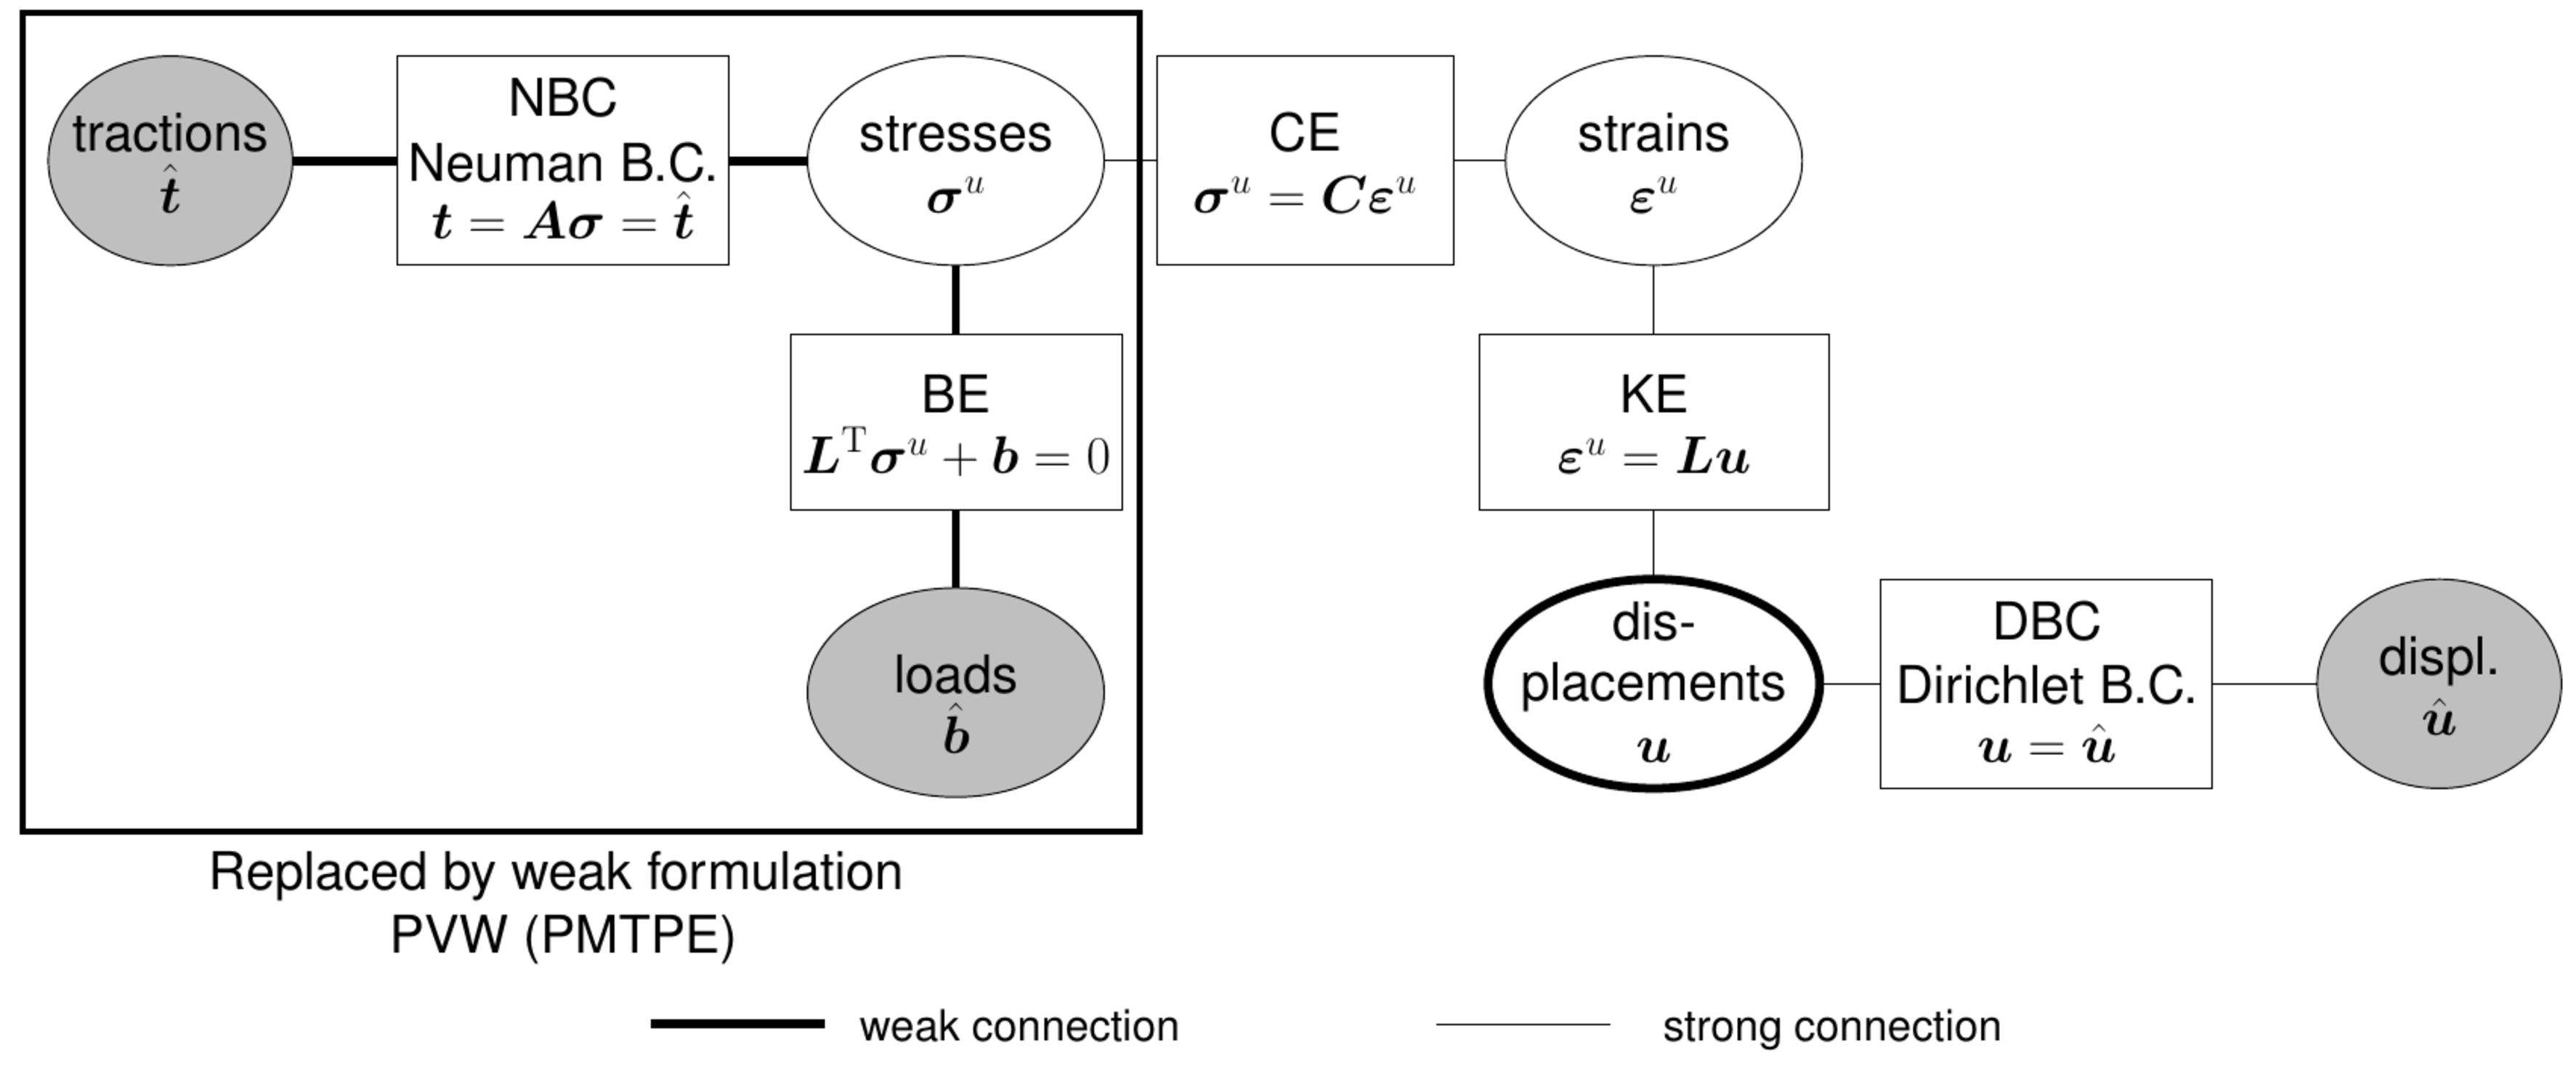
\includegraphics[width=0.8\textwidth]{./fig/pdf/tonti.pdf}
  \caption[Tonti diagram linear]{Tonti diagramm for a linear, small displacement elasticity problem. It classifies variables and equations of the solid mechanics PDEs and helps to derive an appropriate finite element formulation. A classic, displacement based formulation is depicted here.}\label{fig:tonti}
\end{figure} \\
\\
In index-notation, the system of equations to be solved reads
\begin{align}
    & \frac{\partial}{\partial x_i} \sigma_{ij} + \bar{X_j}=0 & in~\Omega_0           \\
    & t_j=n_i \sigma_{ij} = \bar{t}_j                         & on~Neumann~ boundary  \\
  &\sigma_{ij}=\sigma_{ji}\\
  &\sigma_{ij}=C_{ijkl} \epsilon_{kl}\\
  &\epsilon_{ij}=\frac{1}{2} (\frac{\partial u_j}{\partial x_i}+\frac{\partial u_i}{\partial x_j}) \\
    & u_j = \bar{u}_j                                         & on~Dirichlet~boundary 
\end{align}
\\
A system of equations is derived, that can, except for special, very simple cases, not be solved analytically.\\
The finite element method now entails two key ideas. Firstly, instead of a continuous domain, considerations are focused on a finite number of discrete elements("finite elements"). Each Element defines its own function space for the primary variables via the so called shape functions. It is obvious that the thereby introduced limitation of the solution function space will generally not contain the solution to the original problem.  Therefore, as a second step, selected governing equations are "weakened", i.e. they are multiplied by a weighting function and only enforced in an integral sense. For the formulation, presented in Figure~\ref{fig:tonti} the weak form can be formulated as

\begin{align}
  \int_{\Omega}  \underbrace{(\nabla \cdot \stress^{\disp} + \bodyforce)}_{\vec{R}_\mathrm {BE}} ) \cdot \underbrace{\vec{w}}_{\substack{\text{weighting}       \\\text{function}}}~d\Omega +
  \int_{\Gamma_\sigma}  \underbrace{(\nabla \cdot \stress^{\disp} + \bodyforce)}_{\vec{R}_\mathrm{FBC}} )\cdot \underbrace{\vec{w}}_{\substack{\text{weighting} \\\text{function}}}~d\Gamma
  =0~. \label{eq:weighted_residuals}                                                                                                                            
\end{align}


Gauss divergence divergence is subsequently applied for further derivations.
%
\paragraph{Principle of Virtual Work}
Generally, the weight function $\vec{w}$ is arbitrary, and can be chosen freely. If, however, one makes the particular choice of
\begin{align}
  w_\mathrm{i}=\pd u_\mathrm{i} 
\end{align}
work expressions are obtained for the individual terms and the Principle of Virtual Work~(PVW) is derived as (in matrix notation)
\begin{align}
  \int_\Omega \pd \strain^{\disp \mathrm T} \stress^{\disp}~d\Omega                   
  =                                                                                   
  \int_\Omega \pd \disp^{\mathrm T}~d\Omega                                           
  +                                                                                   
  \int_{\Gamma_\sigma} \pd \disp^{\mathrm T} \traction~d\Gamma~. \label{eq:solid_PVW} 
\end{align}


The PVW is valid for arbitrary materials, also for dissipative ones that have no potential.
The finite element formulation is finally derived expressing all terms of the PVW exclusively in the primary variables. To do so, the strong connections of the Tonti diagram are taken advantage of.

\section{Space discretization}\label{sec:space_discretiaztion}
The FEM in solid mechanics is based upon the idea of finding a numerical solution to Equation~\eqref{eq:general_problem_FE} at discrete points, commonly referred to as nodes. Connected nodes form elements, into which the problem domain is partitioned into:
The primary variable on element $e$ is then typically approximated by interpolation functions ~( shape functions ).\\
In this case, the displacement field has been used as the only primary variable, and a local interpolation approach, i.e., the shape functions only have local support, has been utilized.\\
Therefore:
\begin{align}
  \Omega_\mathrm 0   & \approx\cup_\mathrm {e=1}^{nele} \Omega_\mathrm 0^{(e)}~, \\
  \disp(\vec{X},t)   & \approx                                                   
  \disp_\mathrm h^{(e)}(\vec{X},t)=
  \sum_\mathrm {k=1}^{nnod^{(e)}} N_\mathrm k(\vec{X}){d}_\mathrm k(t)~. \label{eq:fe_interpolation} \\
  \vec{x}(\vec{X},t) & \approx                                                   
  \vec{x}_\mathrm h^{(e)}(\vec{X},t)=
  \sum_\mathrm {k=1}^{nnod^{(e)}} N_\mathrm k(\vec{X}){x}_\mathrm k(t)~. \label{eq:fe_interpolation}
\end{align}


\section{Methods of constraint enforcement}\label{sec:constraint_enforcement}
From a mathematical point of view, coupling problems are basically optimization problems with equality constraints. A problem of this kind can generally be formulated as:
\begin{align}\label{eq:optimization_problem}
  \underset{x}{\text{min}}~ & \vec{f(x)}~,   \\
  \text{subjected to }      & \vec{g(x)}=0~. 
\end{align}
Numerous methods have been proposed to solve this kind of problems. Among the most common ones are the Lagrange multiplier approach and the penalty method. This thesis focuses solemnly on the first on, nevertheless a quick introduction into the alternatives shall be provided, so that the pros and cons of each method can be discussed.
\subsubsection{Lagrange multiplier approach}\label{sec:lagrange_multiplier_approach}
The Lagrange multiplier method demands the existence of continuous partial derivatives for both: $\vec{f}$ and $\vec{g}$. It introduces a new variable $\lagvec$, called Lagrange multiplier, and considers the Lagrange function defined as
\begin{align}
  \Lambda(\vec{x},\vec{\lambda})=\vec{f(\vec{x})}+\lambda\cdot\vec{g(\vec{x})}~. 
\end{align}
\\
Solutions of the original problem are stationary points of the Lagrange function. However, not all stationary points yield a solution of the original problem. The method of Lagrange multipliers thus gives a necessary condition. Sufficient conditions can be obtained by surveying the Hessian matrix. Details can be found in any standard mathematical literature concerning optimization theory.
The main advantage of the Lagrange multiplier approach lies in its exact fulfilment of the constraints. Moreover, it is a single step method, meaning that no iterative procedure is necessary to fulfil the boundary conditions.\\
The Lagrange multiplier approach does, however, come with the disadvantage of introducing additional unknowns, as well as worsening the overall system of equations constitution.
\subsubsection{Penalty approach}
A penalty method replaces the constraint problem by a series of unconstrained problems, such that their solutions ideally converge to the solution of the original problem. Basically the series of unconstrained minimization problems can be written as:
\begin{align}
  \text{min}~\Phi(\vec{x}) & =f(\vec{x})+\sigma_\mathrm k \sum_\mathrm {i \in I} g(c_\mathrm i(\vec{x})),~\text{where} \\
  g(c_\mathrm i(\vec{x}))  & = \text{min}(0,ci(x))^2~.                                                                 
\end{align}
They main advantage of the penalty method lies in the fact, that it does not introduce any new unknowns, and thus maintains the positive definiteness of the system matrix. On the other hand, the constraints are not fulfilled exactly. Regarding the choice of $\sigma_\mathrm k$ one has to weight carefully between a more accurate constraint fulfilment and the overall systems constitution since a greater $\sigma_k$ value might enforce the constraints stronger, but can also lead to numerical instabilities.
\subsubsection{Augmented Lagrange}
The Augmented Lagrange method has similarities to the Penalty method. It replaces the constraint optimization problem by a series of unconstrained problems and adds a penalty term to the objective. Moreover, the Augmented Lagrange Method adds yet another term, that mimics a Lagrange multiplier.\\
Starting from the problem defined in Equation~\eqref{eq:optimization_problem}, the approach uses the following unconstrained objective:
\begin{align}
  \mathrm{min}~\boldsymbol{\phi}_\mathrm{k}(\vec{x})=f(\vec{x})+\frac{\mu_\mathrm{k}}{2} \sum_{i\in I} g(c_i)(\vec{x})^2 - \sum_{i\in I} \lambda_i g(c_i)(\vec{x})~. 
\end{align}
After each iteration, not only $\mu_k$, but also the variable $\lambda$ is updated according to the rule
\begin{align}
  \lambda_i \leftarrow \lambda_i-\mu_k c_i(\vec{x}_k)~, 
\end{align}
where $\vec{x}_k$ denotes the solution to the unconstrained problem at the k-th step.\\
The variable $\lambda$ can be regarded as an estimate of the Lagrange multiplier, as introduced in Section~\ref{sec:lag_approach}.\\
Contrary to the Penalty approach, $\mu \rightarrow \infty$ is not required in order to solve the original, unconstrained problem, thanks to the presence of the Lagrange multiplier term. The method is therefore especially favourable due to both, an exact fulfilment of the boundary conditions and no introduction of new Unknowns. It also avoids the ill conditioning of the standard quadratic penalty method.
\subsubsection{Nitsche method}\label{sec:nitsche_method}
The Nitsche Method is closely related to the development of discontinuous Galerkin methods. It has originally been developed as a simple approach to handle Dirichlet boundary conditions, but its real strength lies in the generality with which interface problems can be handled: arbitrary degree of polynomial approximations, arbitrary( shape regular meshes ), even different physical models on either side are possible~\cite{Hansbo2005}.\\
A full introduction is beyond the  scope of this thesis, thorough investigations are provided in~\cite{Nitsche1971} and~\cite{Hansbo2005}.\\
\chapter{The FETI formulation}\label{cha:feti_formulation}
\section{Problem Setup}
The reference problem for all further considerations is described in Figure~\ref{fig:reference_problem}. For the sake of simplicity, a two domain setup shall be considered here, a generalization to an arbitrary number of sub-domains can, however easily be derived.


\begin{figure}[h]
  \centering
  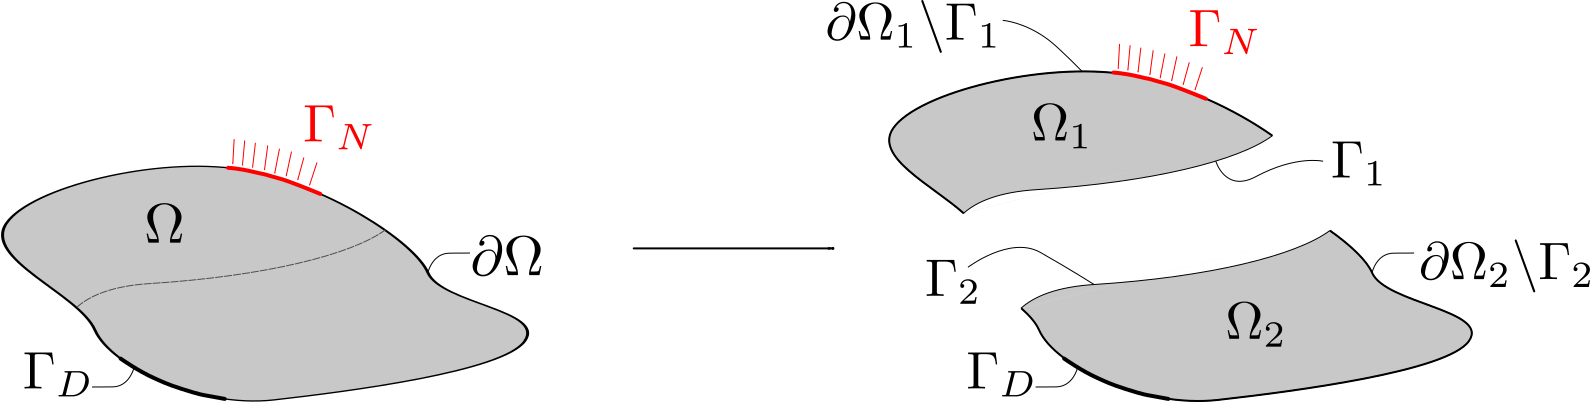
\includegraphics[width=0.8\textwidth]{./fig/eps/drawing1}
  \caption[Domain decomposition reference problem]{Reference problem. The simple case of two substructures is considered here, a generalization to an arbirtray number of substructures can, however, be easily achieved. The domain $\Omega$ is split into the subdomains $\domainone$ and $\domaintwo$ by the interface $\Gamma$. The aim of all DD methods is to distribute those domains to different proccessing nodes and solve the problems as locally as possible. Of course, some interprocessor communication can not be avoided, since information(e.g. the boundary conditions) has to be propagated from one domain to the other. Looking at this example it shall also be noted, that substructuring may introduce so-called "floating substructures", which means substructures can have rigid body modes, although the overall system does not.}\label{fig:reference_problem}
\end{figure}
\begin{figure}[h!]
  \begin{center}
    \includestandalone{\tikzpath/setup_quad4_basic_example}
    \caption[Simple discretized problem]{Basic discretized problem. The setup consists of four substructures, each of which is built up of just one quadrilateral element. Albeit very simple, this example can be used to explain all relevant operators and problems concerning the FETI method. The element/node/dof/Lagrange-multiplier numbering scheme is consistent with the Matlab code developed for this thesis~\cite{FEMAC}. Its is very crucial to note the difference between the global numbering scheme and the substructure-based numbering scheme. }
    \label{fig:simple_discretized_example}
  \end{center}
\end{figure}

\begin{figure}[h!]
  \begin{center}
    \includestandalone{\tikzpath/setup_quad4_basic_example_sub3}
    \caption[Simple discretized problem - detail substructure 3]{Detailed view of the bottom right substructure. Substructure-local dof indices are printed here, since they are used to create the assembly operator $\asmop$. For this particular example, the assembly and trace operator of the bottom right substructure are given in Equation~\eqref{eq:asmop_and_traceop_example}.}
    \label{fig:simple_discretized_example_detail_sub}
  \end{center}
\end{figure}



\section{General}

The simple problem of linear elasticity can be formulated in $\Omega$ as:
\begin{align}
  \dmat{K}\dvec{u}=\dvec{f} 
\end{align}
\\
The FETI-method tears the domain apart, introducing two sub-domains. Thus, a compatibility condition has to be imposed, linking them together. The FETI method enforces this compatibility by the Lagrange multiplier approach(see Section~\ref{sec:lagrange_multiplier_approach}). One can thus write:
\begin{align}
  \idone{\dmat K}\idone{\dvec u}                   & =\idone{\dvec f}\label{eq:elasticity_equation_domain1} \\
  \idtwo{\dmat K}\idtwo{\dvec u}                   & =\idtwo{\dvec f}\label{eq:elasticity_equation_domain2} \\
  (\dvec{\lambda},\dvec{\idtwo u}-\dvec{\idone u}) & =0\label{eq:compatibility_constraint}                  
\end{align}
\\
In contrast to e.g. the mortar method, the FETI approach, enforces Equation~\eqref{eq:compatibility_constraint} not in an integral, but in a point-wise sense. This does not introduce errors, since only conforming meshes are considered here.\\
For an arbitrary number of sub-domains Equations~\eqref{eq:elasticity_equation_domain1}-\eqref{eq:compatibility_constraint} can be equivalently formulated as
\begin{align}
  \ids{\stiffmat} \ids{\dispvec} = \ids{\dvec{f}}+{\ids{\traceop}}^T {\ids{\asmop}}^T \lagvec\label{eq:basic_subdomain_equation} \\
  \sum_s \ids{\traceop} \ids{\asmop} \ids{\dispvec}=0\label{eq:basic_subdomain_equation_asm}                                     
\end{align}
where $\ids{\asmop}$ is a substructure-based, boolean assembly operator, who's rows correspond to the global Lagrange multipliers, and who's columns relate to the substructure-based interface-dofs. A negative sign is used, when the Lagrange multiplier connects to a substructure with a smaller ID, otherwise a positive sign is entered. This reflects the condition from Equation~\eqref{eq:compatibility_constraint}.\\
The trace operators $\ids{\traceop}$, map the columns of $\ids{\asmop}$ to a substructure-based total dof numbering scheme.
\\
For the basic example as described in Figure~\ref{fig:simple_discretized_example} the operators $\asmop$ and $\traceop$ for the bottom left substructure(isolated in Figure~\ref{fig:simple_discretized_example_detail_sub}) are given as

\begin{equation}
  \begin{array}{lc}
    \texttt{$B^{(3)}=$} & \kbordermatrix{\text{} & 1 & 2 & 3 & 4 & 5 & 6\cr 
    1&\0&\0&\0&\0&\0&\0\cr
    2&\0&\0&\0&\0&\0&\0\cr
    3&\0&\0&\0&\0&\0&\0\cr
    4&\0&\0&\0&\0&\0&\0\cr
    5&\0&\0&-1&\0&\0&\0\cr
    6&\0&\0&\0&-1&\0&\0\cr
    7&\0&\0&\0&\0&\0&\0\cr
    8&\0&\0&\0&\0&\0&\0\cr
    9&\0&\0&\0&\0&\0&\0\cr
    10&\0&\0&\0&\0&\0&\0\cr
    11&\0&\0&-1&\0&\0&\0\cr
    12&\0&\0&\0&-1&\0&\0\cr
    13&\0&\0&\0&\0&-1&\0\cr
    14&\0&\0&\0&\0&\0&-1\cr
    15&\0&\0&\0&\0&\0&\0\cr
    16&\0&\0&\0&\0&\0&\0\cr
    17&1&\0&\0&\0&\0&\0\cr
    18&\0&1&\0&\0&\0&\0\cr
    19&\0&\0&1&\0&\0&\0\cr
    20&\0&\0&\0&1&\0&\0}\\
  \end{array},~~
  \begin{array}{lc}
    \texttt{$\traceop^{(3)}=$} & \kbordermatrix{\text{} & 1 & 2 & 3 & 4 & 5 & 6 & 7 & 8\cr 
    1&1&\0&\0&\0&\0&\0&\0&\0\cr
    2&\0&1&\0&\0&\0&\0&\0&\0\cr
    3&\0&\0&\0&\0&1&\0&\0&\0\cr
    4&\0&\0&\0&\0&\0&1&\0&\0\cr
    5&\0&\0&\0&\0&\0&\0&1&\0\cr
    6&\0&\0&\0&\0&\0&\0&\0&1}\\
  \end{array}
  \label{eq:asmop_and_traceop_example}
\end{equation}
\\
The basic idea of FETI now is to reduce the substructure domain problems to a connected interface problem. This can be achieved very elegantly, by rearranging the basic equations \eqref{eq:basic_subdomain_equation}-\eqref{eq:basic_subdomain_equation_asm} and was first described in~\cite{Farhat1991}.
\\
One  should note, that a solution to Equation~\eqref{eq:basic_subdomain_equation} can only exist if $(\ids{\dvec{f}}+{\ids{\traceop}}^T {\ids{\asmop}}^T \lagvec)$ is orthogonal to the null-space of $\stiffmat$.
\\
\section{Interface reduction}\label{sec:interface_reduction}
As mentioned FETI is a reduction technique that solves for the interface unknowns only. After the interface solution has been obtained, the global solution will be recovered.\\
This section is denoted to an step by step explanation of the reduction and subsequent recovery process. We will end up with a system of Equations in the interface unknowns(ans possibly some rigid body modes) only. The process of solving that system will be discussed in Section~\ref{cha:feti_solvers}.
\\
\\
We begin considerations by a reformulation of Equation\eqref{eq:basic_subdomain_equation} as:
\begin{align}
  \ids{\dispvec}=\inv{\ids{\stiffmat}} (\ids{\dvec{f}}+\tp{\ids{\traceop}} \tp{\ids{\asmop}} \lagvec) 
  \label{eq:displacement_recovery}                                                                    
\end{align}
However, as will be explained in Section~\ref{sec:natural_subspace}, for static problems it is required to search for $\lagvec$ in the so-called natural subspace, which is is the rigid body mode free space. Thus,
\begin{align}
  \ids{\dispvec}=\inv{\ids{\stiffmat}} (\ids{\dvec{f}}+\tp{\ids{\traceop}} \tp{\ids{\asmop}} \lagvec) + \ids{\nullspacemat} \ids{\rmodevec} 
  \label{eq:interpolation_full_displacement}                                                                                                
\end{align}
where $\ids{\nullspacemat}$ denotes the nullspace of $\ids{\stiffmat}$ and $\ids{\rmodevec}$ are the generalized coordinates for the interpolation. It should be noted that for the iterative solution process that will follow, a practical implementation will involve a matrix factorization anyway. The nullspace thus comes as a by-product for free.
\\
\\
Inserting Equation~\eqref{eq:interpolation_full_displacement} into Equation~\eqref{eq:basic_subdomain_equation_asm} gives
\begin{align}
    & \sum_s \ids{\asmop} \ids{\traceop} \big(\inv{\ids{\stiffmat}} (\ids{\dvec{f}}+\tp{\ids{\traceop}} \tp{\ids{\asmop}} \lagvec)+\nullspacemat\ids{\rmodevec}\big)=0\text{   or} \\
    & \underbrace{(\sum_s \underbrace{ \ids{\asmop}                                                                                                                                             
  \underbrace{\ids{\traceop} \inv{\ids{\stiffmat}} \tp{\ids{\traceop}}}_{\ids{\dmat{F}}}
  \tp{\ids{\asmop}} }_{\asmids{\locdualschur}} }_{\dmat{F}} ) \lagvec +
  \sum_s \underbrace{\ids{\asmop}  \ids{\traceop} \ids{\nullspacemat}}_{\ids{\rmodespace}} \ids{\rmodevec}
  =
  \underbrace{\sum_s \ids{\asmop}  \ids{\traceop} \inv{\ids{\stiffmat}}  \ids{\forcevec}}_{-\dvec{d}}
\end{align}
\\
where the abbreviations $\ids{\locdualschur}$ for the local dual schur complement, $\asmids{\locdualschur}$ for the assembled local dual schur complement, $\rmodespace$ for the rigid body mode space and $\ifacedispvec$ for the condensed interface displacements have been introduced.\\
\\
So far, the system is under-determined, since we only have two equations, but three unknowns. However, a third equation can be derived by looking at Equation~\ref{eq:basic_subdomain_equation}. If $\ids{\stiffmat}$ is singular, a solution can only exist if $(\ids{\dvec{f}}+{\ids{\traceop}}^T {\ids{\asmop}}^T \lagvec)$ has no component in the Nullspace $\nullspacemat$:
\begin{align}
    & \tp{\ids{\nullspacemat}}(\ids{\dvec{f}}+{\ids{\traceop}}^T {\ids{\asmop}}^T \lagvec)=0\text{  or}\label{eq:reason_natural_subspace} \\
    & \underbrace{\tp{\ids{\nullspacemat}} \ids{\dvec{f}}}_{\tp{\ids{\dvec{e}}}} =                                                        
  \underbrace{\tp{\ids{\nullspacemat}}  \tp{\ids{\traceop}} \tp{\ids{\asmop}}}_{\tp{\ids{\rmodespace}}} \lagvec  
\end{align}
where the abbreviation $\dvec{e}$ for the components of the external forces in the rigid body mode space has been established.
\\
Moreover, we can introduce
\begin{align}
  \ids{\locschur}&=\ids{\stiffmat_{bb}}-\ids{\stiffmat_{bi}}\pinv{\ids{\stiffmat_{ii}}}\ids{\stiffmat_{ib}}\label{eq:locschur} \\
  \asmids{\locschur}&=\tp{\asmop} \left( \ids{\locschur} \right) \asmop \\
  \locschur&= \sum_s \asmids{\locschur}
\end{align}
as the local schur operator, assembled local schur operator and global schur operator respectively.\\
Throughout this thesis $\ids{(\cdot)}$ will be used for substructure local quantities and $\asmids{(\cdot)}=\sum_s \ids{\asmop}\ids{\traceop} \ids{(\cdot)} \tp{\ids{\traceop}} \tp{\ids{\asmop}}$ denotes the assembled local quantity.

\section{Matrix notation}\label{sec:matrix_notation}
Putting all previously derived Equations together, one can finally write the basic FETI Problem in matrix notation as:
\begin{align}
  \begin{bmatrix}
  \locdualschur    & \rmodespace \\
  \tp{\rmodespace} & \dmat{0}    
  \end{bmatrix}
  \begin{bmatrix}
  \lagvec\\
  \rmodevec
  \end{bmatrix}
  =
  \begin{bmatrix}
  \ifacedispvec\\
  \dvec{e}
  \end{bmatrix}
  \label{eq:feti_equation_system}
\end{align}
\\
Where
\begin{align}
  %\ids{\nullspacemat}&=ker(\ids{\stiffmat}) \\
  \dmat{e}      & =\tp{\begin{bmatrix} \cdots,\tp{\ids{\forcevec}} \ids{\nullspacemat},\cdots \end{bmatrix}}   \\
  \rmodespace   & =\begin{bmatrix} \cdots,\ids{\asmop}\ids{\traceop}\ids{\nullspacemat},\cdots \end{bmatrix}   \\
  \locdualschur & =~~\sum_s \ids{\asmop} \ids{\locdualschur} \tp{\ids{\asmop}} \label{eq:definition_dualschur} \\
  \ifacedispvec & =-\sum_s \ids{\asmop}  \ids{\traceop} \inv{\ids{\stiffmat}}  \ids{\forcevec}                 
\end{align}
and $\lagvec$ are the unknown interface forces, $\rmodevec$ the rigid body mode components respectively.
\\
\section{The natural subspace}\label{sec:natural_subspace}
As was explained in \eqref{eq:reason_natural_subspace}, classical FETI formulation encounters a problem for static calculations if the local stiffness matrix is singular. In that case, we required
\begin{align}
    & \tp{\ids{\nullspacemat}}(\ids{\dvec{f}}+{\ids{\traceop}}^T {\ids{\asmop}}^T \lagvec)=\dvec{0}%\label{eq:reason_natural_subspace} 
\end{align}
where $\asmop$ is the substructure based boolean assembly operator, introduced in Equation~\eqref{eq:basic_subdomain_equation}, consisting of $0,+1,-1$, defined such that the continuity conditions for each Lagrange multiplier is ensured(see~Equation~\eqref{eq:compatibility_constraint})
\\
We had solved this problem by prescribing the
\begin{align}
  \tp{\rmodespace} \totalgap_i =0           
  \label{eq:orthogonality_natural_subspace} 
\end{align}
\\
Inserting Equation~\eqref{eq:totalgap} one can thus write
\begin{align}
  \tp{\rmodespace} (\ifacedispvec-\locdualschur \lagvec_i - \rmodespace \rmodevec_i ) =0 
\end{align}
\\
which can easily be reformulated to
\begin{align}
  \tp{\rmodespace} \underbrace{(\ifacedispvec- \locdualschur \lagvec_i)}_{\resvec_i} - \tp{\rmodespace} \rmodespace \rmodevec_i =0 
\end{align}
\\
Solved for $\rmodevec_i$ this gives
\begin{align}
  \rmodevec_i=\inv{(\tp{\rmodespace}\rmodespace)}\tp{\rmodespace}\resvec_i 
  \label{eq:r_to_alpha}                                                    
\end{align}
\\
Inserting Equation~\eqref{eq:r_to_alpha} into Equation~\eqref{eq:totalgap} gives
\begin{align}
  \totalgap_i & =\resvec_i-\rmodespace \inv{(\tp{\rmodespace}\rmodespace)}\tp{\rmodespace}\resvec_i                       \\
              & =\underbrace{(\eyemat-\rmodespace \inv{(\tp{\rmodespace}\rmodespace)}\tp{\rmodespace})}_{\projn}\resvec_i 
\end{align}
where by looking at the equation, $\projn$ can be interpreted as a projection operator, that removes all rigid body components from $\resvec_i$.
\\
As first described in \cite{Farhat1992}, and further investigated in \cite{RixenPhD} it is often advantageous to choose $\totalgap_i$ to be not simply orthogonal, but A-orthogonal to a matrix A:
\begin{align}
  \tp{\rmodespace} \scalemat \totalgap_i =0 
\end{align}
\\
which leads to the following expression for the natural subspace projector
\begin{align}
  \tp{\projn}=\eyemat-\scalemat\rmodespace \inv{(\tp{\rmodespace}\scalemat\rmodespace)}\tp{\rmodespace} 
\end{align}

\paragraph{Choices for $\dmat{A}$}
The equation for the natural subspace projector above has introduced the matrix $\scalemat$. It has been shown in\cite{RixenPhD} that this matrix plays the role of a preconditioner for the coarse grid displacements.
Ideally, the preconditioner used for the Conjugate Gradient iterations should be taken for $\scalemat$.
\\
The Equations in the previous chapter show that the Lagrange multipliers are corrected by a step of $\scalemat \rmodespace$ at every Conjugate Gradient iteration.
From a dimensional point of view, one can thus argue that since $\rmodespace$ represents restrictions on the displacement modes, $\scalemat$ should represent a stiffness matrix. Particularly, since the product represents interface forces due to rigid body modes, the ideal choice for $\scalemat$ is the preconditioner.\\
However, choosing the preconditioner typically introduces a significant fill-in in the inversion of $\rmodespace \scalemat \tp{\rmodespace}$.\\
The bottom line is that in most cases simply choosing $\scalemat=\eyemat$ is the more efficient option. During this thesis, this choice has been retained.

\section{Residuum formulation}\label{sec:residuum_formulation}
The natural solver choice for the FETI problem is the Conjugate Gradient method. This chapter aims at formulating the CG algorithm specifically for the FETI problem. Some alternations to the classical CG notation will be done to ensure parallel efficiency of the method.\\
\\
The CG algorithm consists of three main points. Firstly new search directions are created, these search directions are then updated through orthogonalization to the previous one, and finally an optimal step length is determined by minimizing the residual error along this direction. In practice, Orthogonalization is performed with regards to all previous search directions due to the finite precision of the machine.
\\
The first question is therefore, how to derive the search directions. Since FETI operates on interface forces as primary variables, we need an update for the force vector.
\\
For any given approximation $\lagvec$ to the interface force solution one can calculate the resulting gap between the substructures as
\begin{align}
  \totalgap_i=\sum_s \ids{\asmop}\ids{\dispvec}=\ifacedispvec-\locdualschur \lagvec_i - \rmodespace \rmodevec = \dvec{0} \label{eq:totalgap} 
\end{align}
\\
The gap, projected to the natural subspace can thus be written as
\begin{align}
  \resvec_i=\tp{\projn}(\ifacedispvec-\locdualschur\lagnvec_i) 
\end{align}
where the rigid body mode component vanished due to the very definition of the natural subspace projector $\projn$.
\\
The idea now it to estimate the interface forces associated with displacement of that value by a preconditioning step:
\begin{align}
  \dvec{z}_i=\scaled{\locschur}\resvec_i 
\end{align}
\\
Since the local schur operator has full rank, one again need a projection to the natural subspace to eliminate all rigid body mode components.
\begin{align}
  \dvec{w}_i=\projn\dvec{z}_i 
\end{align}
\\

The dual schur operator $\locdualschur$ is used to calculate the interface displacements related to this forces as
\begin{align}
\dvec{q}_i = \locdualschur \sdirnspace_i
\end{align}


After full orthogonalization of the search direction a line-search is performed to minimize the energy expression. The Lagrange multiplier is then updated as

\begin{align}
\delta_i&=\tp{\dvec{q}_i}\dvec{w}_i\\
\gamma_i&=\tp{\dvec{r}_i} \dvec{z}_i\\
\lagfvec_{i+1}&=\lagfvec_i+(\gamma_i/\delta_i)\sdirnspace_i 
\end{align}
\\
The resulting gap to to the updated force does not need to be explicitly computed, but instead it can be updated too as

\begin{align}
  \resvec_{i+1}=\resvec_i-(\gamma_i/\delta_i)\tp{\projn}\sdirnspacecspace_i 
\end{align}
\\
The process is then repeated until satisfying convergence has been obtained.
The full solution for lambda is then recovered as
\begin{align}
  \lagvec=\lagvec_0+\lambda_ F 
\end{align}
The displacements can finally be recovered by Equation~\eqref{eq:displacement_recovery}.

\section{Preconditioners}\label{sec:precond}
As will be explained in Chapter~\ref{cha:iterative_solvers}, iterative solution techniques typically use preconditioners to accelerate convergence.
As can be seen from the formulation above preconditioner in the context of FETI is an approximation to the operator
\begin{align}
\sum_s \ids{\asmop} \inv{\ids{\stiffmat}} \tp{\ids{\asmop}}
\end{align}
The natural choice for this problem in the FETI formulation can be identified as
\begin{align}
\inv{\precond}=\sum_s \ids{\asmop} \ids{\traceop} \ids{\locschur} \tp{\ids{\traceop}} \tp{\ids{\asmop}}
\end{align}
where the schur complement $\locschur$ is defined as
\begin{align}
\ids{\locschur}=\ids{\stiffmat}_{bb}-\ids{\stiffmat}_{bi} \pinv{\ids{\stiffmat}_{ii}} \ids{\stiffmat}_{ib}
\label{eq:locschur2}
\end{align}
This version of the preconditioner is typically denoted as Dirichlet preconditioner in the literature.\\
The pseudo inversion of $\pinv{\ids{\stiffmat}}$ is costly and introduces a lot of non-zero entries in the preconditioner matrix. Therefore~\cite{Farhat1991} proposed to neglect the second term in Equation~\eqref{eq:locschur2}, which results in the o called lumped preconditioner. One can summarize
\begin{align}
\inv{\precond}_D&=\sum_s \ids{\asmop} \ids{\traceop}
\left(  \ids{\stiffmat}_{bb}-\ids{\stiffmat}_{bi} \pinv{\ids{\stiffmat}_{ii}} \ids{\stiffmat}_{ib}  \right)
\tp{\ids{\traceop}} \tp{\ids{\asmop}} &\text{ ... Dirichlet Preconditioner} \\
\inv{\precond}_L&=\sum_s \ids{\asmop} \ids{\traceop}
\pinv{\ids{\stiffmat}_{ii}}
\tp{\ids{\traceop}} \tp{\ids{\asmop}} &\text{ ... Lumped Preconditioner}
\label{eq:precond}
\end{align}
However, this definition of the preconditioner has been shown to be not consistent in~\cite{Rixen1999a} for the case where crosspoints are present. A Crosspoint is a point, of the mesh where more than two substructures meet. An example would be node 5 in Figure~\ref{fig:simple_discretized_example} where all four substructures meet. It is obvious that our definition of the Lagrange multipliers introduces a redundancy in the Equations, since one could simply drop the four diagonal Lagrange multipliers, and still the problem would be fully determined. The identifications and removal of redundant Lagrange multipliers, however, is cumbersome and inefficient.\\
From a mechanical point of view, the problem arises when updating the interface displacements in the Conjugate Gradient. If one dof carries more than one Lagrange multiplier, than its displacement is multiply updated and the update steps typically contradict on another in a non-converged situation.\\
A simple and effective approach to eliminates this problem is Multiplicity Scaling. It can be formulated as
\begin{align}
\inv{\precond}_{D}&=\sum_s \ids{\dmat{D}} \ids{\asmop} \ids{\traceop}
\ids{\locschur}
\tp{\ids{\traceop}} \tp{\ids{\asmop}} \ids{\dmat{D}} &\text{ ... Dirichlet Preconditioner} \\
\inv{\precond}_{L}&=\sum_s \ids{\dmat{D}}  \ids{\asmop} \ids{\traceop}
\pinv{\ids{\stiffmat}_{ii}}
\tp{\ids{\traceop}} \tp{\ids{\asmop}} \ids{\dmat{D}}  &\text{ ... Lumped Preconditioner}
\label{eq:precond_mscaled}
\end{align}
where $\ids{\dmat{D}}$ is a substructure based diagonal scaling matrix, that holds the multiplicity of the corresponding interface dofs. As multiplicity of a dof we define the number of Lagrange multiplier related to that dof. This multiplicity can be derived very elegantly as
\begin{align}
\dmat{D}&=\frac{1}{2} \tp{\asmop}\asmop\\
\asmop&=\sum_s \ids{\asmop} \ids{\traceop}
\end{align}
\\
Another inconsistency, when it comes to preconditioners are heterogeneities across substructure interfaces. Similarly to the considerations above, a scaling approach can be defined too, according to

\begin{align}
\inv{\precond}_{D}&=\sum_s \ids{\dmat{\beta}} \ids{\asmop} \ids{\traceop}
\ids{\locschur}
\tp{\ids{\traceop}} \tp{\ids{\asmop}} \ids{\dmat{\beta}} &\text{ ... Dirichlet Preconditioner} \\
\inv{\precond}_{L}&=\sum_s \ids{\dmat{\beta}}  \ids{\asmop} \ids{\traceop}
\pinv{\ids{\stiffmat}_{ii}}
\tp{\ids{\traceop}} \tp{\ids{\asmop}} \ids{\dmat{\beta}}  &\text{ ... Lumped Preconditioner} \\
\beta^{(s),i} &= diag(\stiffmat_{bb}^{(s),i}) \left[  \sum_{r:\Gamma_I^i \subset \{  \Gamma_I \cap \Gamma_I^{(r)}  \} } diag(\stiffmat_{bb}^{(r),i})  \right]^{-1} &
\label{eq:precond_kscaled}
\end{align}
Rixen and Farhat introduced this approach as "Superlumped Smoothed Preconditioner". In the literature the more descriptive term "K-scaling" is often used.\\
Both scaling approaches introduced here are appealing since they do not introduce a significant extra cost, while drastically improving the solver performance, especially for the case with high heterogeneities across the interface. The policy in this thesis, that can also be recommended with clear considence as a standard approach, therefore is to always use both of these scaling types combined. Exceptions(see Chapter~\ref{cha:numerical_assesment}) will be explicitly mentioned.


\section{Scalability}\label{sec:scalability}
The main goal of a DD algorithm is scalability. Generally, one can distinguish numerical scalability and parallel scalability. In iterative DD methods as FETI, numerical scalability is given if the condition number after the preconditioning step grows weakly with the ratio of the sub-domain-size $h$ to the overall size $H$.\\
For unpreconditioned interface problems \cite{Mandel1996} have shown, that the condition number grows asymptotically
\begin{align}
  \condnum=\myorder{\frac{H}{h}}            
  \label{eq:condnum_without_natural_cspace} 
\end{align}
which makes algorithms like that useless for real engineering problems. The authors in \cite{Mandel1996} have proven mathematically, that using sub-domain-based Dirichlet operators as pre-conditioners results in a condition number of the natural coarse problem of
\begin{align}
  \condnum=\myorder{1-log^\beta(\frac{H}{h})} 
\end{align}
\linebreak
It is important to note, that the numerical scalability of the FETI-1 method can be traced back to the inherent problem of the natural coarse space.
This gives rise to a problem, when it comes to structural dynamics calculations. As \cite{Farhat1998} writes, and as it was shown in Section~\ref{sec:natural_subspace} the natural coarse problem was introduced due to a potential singularity of the substructure stiffness matrices.\\
This singularity, however, its no longer present in dynamic calculation, since an implicit time integrator typically leads to a system of equations that is governed by substructure matrices of the form
\begin{align}
  \ids{\dmat{A}}=\ids{\dmat{M}}+\zeta \Delta t^2\ids{\dmat{K}} 
\end{align}
Since $\ids{\dmat{M}}$ is positive definite and $\dmat{K}$ is positive semi definite, any linear combination of the two is also positive definite and thus invertible. However, as Farhat\cite{Farhat1998} wrote, loosing the projector $\projn$ means loosing its mechanism of propagating the error globally, which was the basis of the scalability considerations performed in \cite{Farhat1998}, see also Section~\ref{sec:scalability}.\\
Without the natural coarse problem,however, the conditioning properties are thrown back to Equation~\eqref{eq:condnum_without_natural_cspace}
A solution to this problem is the introduction of an auxiliary coarse problem, which will leads to the FETI-2 methods described in Section~\ref{sec:feti2}.
\chapter{Iterative Solution techniques}\label{cha:iterative_solvers}
It has already been outlined, that the goal of FETI methods is parallelism. The approach was to solve local domain-wise problems on different computing nodes. A serial interface problem then remains to connect the local problems. It thus comes natural, that the solution process of this problem should also be parallelized, otherwise scalability will be quite poorly due to Amdahl's law.\\
Direct solver thus can not be used as they are inherently serial. We chose to use iterative solver instead, which will be discussed in this chapter.

\section{Theory}\label{sec:iterative_theory}
For the purpose of this introduction, and to be consistent with the notation from~\cite{Spillane2016}, considerations will be generalized to the linear system
\begin{align}
\dmat{A} \dvec{x} = \dvec{b}
\label{eq:basic_linear_equation}
\end{align}
As described in~\cite{Kaniel1966}\cite{Saad2003}, the convergence properties of an iterative method applied to a system of type~\eqref{eq:basic_linear_equation} depend on the condition number of the matrix $\dmat{A}$.\\
We will see in Chapter~\ref{cha:numerical_assesment}, that substructuring often leads to very ill-conditioned problems. One therefore typically solves the related problem
\begin{align}
\dmat{H}\dmat{A} \dvec{x} = \dmat{H}\dvec{b}
\label{eq:preconditioned_linear_equation}
\end{align}
instead.\\
\\
The matrix $\dmat{H}$ is thereby chosen as an approximation to the inverse of $\dmat{A}$, which significantly improves the condition number of the new iteration matrix $\dmat{H}\dmat{A}$.\\
The crucial part therefore is, of course, the choice of an appropriate preconditioner. A simple, but not very effective approach could be the inverse of the diagonal of $\dmat{A}$. Other types are deflation, augmentation as well as balancing. For the FETI method, the natural choice, however, is projection. The reason for this is explained in~\cite{Farhat1991}.\\
The idea is simple. One assumes that the bad condition number of the matrix is caused by just a little fraction of the full eigenvalue spectrum. One therefore tries to identify these "bad" eigenmodes and create a so called "auxiliary coarse space(deflation space)" with those modes. The problem is then solved directly within this small subspace, before the iterative scheme continues in the remaining space, orthogonal to the deflation space. If the deflation space is chosen right, the convergence properties are significantly improved.\\
\section{The Conjugate Gradient algorithm}\label{sec:cg}
The most prominent iterative solver is the Conjugate Gradient method. We will see, that the choice of CG comes natural with the FETI formulation. This section is denoted to a formulation of several special variants of CG that we will use in Chapter~\ref{cha:feti_solvers}. Considerations are limited to Preconditioned Conjugate Gradient methods.


%\subsection{The Preconditioned Conjugate Gradient algorithm}\label{sec:pcg}
%\begin{figure}[h!]
%	\begin{center}
%        \subimport{./}{\tikzpath/CG/CG}
%        \caption[Structogram Preconditioned Conjugate Gradient algorithm]{Structogram of the Preconditioned Conjugate Gradient algorithm. The purpose of the preconditioner is to improve the eigenvalue spectrum of the iteration matrix, thus accelerating convergence.}
%		\label{struk:PCG}
%    \end{center}
%\end{figure}


\subsection{The Projected Preconditioned Conjugate Gradient algorithm}\label{sec:ppcg}
The PPCG algorithm introduces both a left preconditioner $\dmat{H}$ as well as a right preconditioner $\dmat{\Pi}$, where the latter one can be interpreted as an A-orthogonal projection to a subspace defined by U:
\begin{align}
\dmat{\Pi}=\eyemat-\dmat{U}(\tp{\dmat{U}}\dmat{A}\dmat{U}  )\tp{\dmat{U}}\dmat{A}
\end{align}
The derivation of the projector equation was outlined in Section~\ref{sec:natural_subspace}.
\\
The general form of a PPCG algorithm is depicted in Figure~\ref{struk:PPCG}

\begin{figure}[h!]
	\centering
        \subimport{./}{\tikzpath/CG/PPCG}
        \caption[Structogram Projected Preconditioned Conjugate Gradient]{Structogram of the Projected Preconditioned Conjugate Gradient. Compared to the PCG algorithm,  the solution is searched for in a subspace, orthogonal to a chosen space $\dmat{U}$. The idea is to put "bad modes" into this space, to improve convergence. }
		\label{struk:PPCG}
\end{figure}

From the formulation above it is obvious, that the choice of the coarse space is essential. Naturally, further augmenting the space $\dmat{U}$ leads to better convergence. In the limit, if all vectors are incorporated into $\dmat{U}$ a direct solution method is retrieved, and convergence is achieved in one step. However, building the projector $\dmat{\Pi}$ entails the factorization of $\dmat{\tp{U} A U}$. A reasonable compromise should thus be found.\\
A useful tool for convergence studies are error estimators. In \cite{Kaniel1966} the following a posterior one is introduced for the PCG algorithm:
\begin{align}
\frac{\norm{\dvec{x}_*-\dvec{x}_i   }_A}{\norm{\dvec{x}_*-\dvec{x}_0}_A} =
2 \Bigg [ \frac{ \sqrt{\lambda_{\dmat{H A},max}/\lambda_{\dmat{H A},min}}-1 }{ \sqrt{\lambda_{\dmat{H A},max}/\lambda_{\dmat{H A},min}}+1 } \Bigg ]^i
\label{eq:errro_estimate_pcg}
\end{align}
Here, $\dvec{x}_*$ denotes the final, converged solution, $\lambda_{\dmat{H A},max}$ and $\lambda_{\dmat{H A},min}$ denote the maximal and minimal value of the Preconditioned matrix $\dmat{A}$ respectively.
\\
Equivalently an estimate for the PPCG algorithm can be derived as

\begin{align}
\frac{\norm{\dvec{x}_*-\dvec{x}_i   }_A}{\norm{\dvec{x}_*-\dvec{x}_0}_A} =
2 \Bigg [ \frac{ \sqrt{\lambda_{\dmat{H A \Pi},max}/\lambda_{\dmat{H A \Pi},min}}-1 }{ \sqrt{\lambda_{\dmat{H A \Pi},max}/\lambda_{\dmat{H A \Pi},min}}+1 } \Bigg ]^i
\end{align}
\\
The function described by this formula is visualized in Figure~\ref{fig:error_estimation_pcg}. The figure shows, that the convergence properties are extremely sensible to the condition number of the projected, preconditioned operator. The proposed strategy in the PPCG algorithm thus is to identify all extreme, isolated eigenvalues an use their corresponding eigenvectors to built the coarse space. The remaining iteration matrix will thus show a lower condition number, which should be reflected higher convergence rates.
\begin{figure}[h!]
	\begin{center}
	    %\fbox{\subimport{./}{./fig/tikz/study_inclusion.tex}}
        \subimport{./}{\tikzpath/error_estimationPCG}
        \caption[A posteriori error estimation PCG]{A posteriori error estimation for the PCG algorithm according to Equation~\eqref{eq:errro_estimate_pcg}. As expected, a condition number of 1 leads to a direct solution. The graph shows that an increasing eigenvalue ratio, drastically worsens performance.}
		\label{fig:error_estimation_pcg}
    \end{center}
\end{figure}


\subsection{The Multi Preconditioned Conjugate Gradient algorithm}\label{sec:mpcg}
The main idea of the Multi Preconditioned Conjugate Gradient algorithm is intuitive. It is designed for problems, where the preconditioner can be written as a sum of local contributions. The approach is straightforward. Instead of adding all local contributions together, each local direction is solved for independently. Therefore, in every iteration the algorithm searches for an optimal step in a space of dimension $\#~substructures$. Of course, the cost of one iteration is significantly higher than for FETI-2, but the hope is, that the overall number of iterations can be significant reduced, especially for problems with very local phenomena like jumps in the material coefficients. The MMPCG algorithm is summarized in Figure~\ref{struk:MPPCG}.

\begin{figure}[h!]
	\centering
        \subimport{./}{\tikzpath/CG/MPPCG}
        \caption[Structogram Multi Preconditioned Projected Conjugate Gradient]{Structogram of the Multi Preconditioned Projected Conjugate Gradient. The main difference compared to the PPCG algorithm as described in Figure~\ref{struk:PPCG} is that a whole set of search directions is used in each iteration. }
		\label{struk:MPPCG}
\end{figure}


\subsubsection{The Adaptive Multi Preconditioned Conjugate Gradient Algorithm}\label{sec:ampcg}
The previous section has introduced the Multi Preconditioned Conjugate Gradient method. Therein, each iteration will give significantly better results than a simple PCG one, thanks to the increased iteration space. However, with a growing number of substructures, solving in the growing search space can become quite expensive.\\
Remembering that MMPCG was derived as a method for problems, where the preconditioner can be written as a sum of contributions, it seems rational to assume that some local contributions are less important than others.\\
The idea of Adaptive MMPCG therefore is to identify the important directions, built the search space with them, and to sum the not-so-important directions simply up, like in PCG.\\
\\
To do so, a method must be derived that determines the importance of a search direction. Of course the cost of this calculation must be kept low to get an effective improvement over MPPCG.\\
An approach to do so, was first described in \cite{Spillane2013} and further investigated in \cite{Spillane2016}.\\


First of all, an a priori error estimate should be derived~\cite{Axelsson2001}.\\
We know that
\begin{align}
\dvec{x}_* =\dvec{x}_0 + \sum_{j=0}^{n-n_0-1}\alpha_i \dvec{p}_j = \dvec{x}_i + \sum_{j=i}^{n-n_0-1} \alpha_j \dvec{p}_j
\end{align}
where $\dvec{x}_*$ is the actual solution.
Since, by construction, search directions are $\dmat{A}$-orthogonal one can write
\begin{align}
\norm{\dvec{d}_i}_{\dmat{A}}^2=
 \norm{\dvec{x}_{*}-\dvec{x}_i}_{\dmat{A}}^2=\sum_{j=i}^{n-n_0-1} \alpha_j^2 \norm{\dvec{p}_i}_{\dmat{A}}^2
\end{align}
Simple subtraction finally gives:
\begin{align}
\norm{\dvec{d}_i}_{\dmat{A}}^2=\norm{\dvec{d}_{i-1}}_{\dmat{A}}^2-\alpha_{i-1}^2 \norm{\dvec{p}_{i-1}}_{\dmat{A}}^2
\end{align}
\\
The authors in~\cite{Axelsson2001} now use this to derive the a-posteriori error estimate as
\begin{align}
\frac{\norm{\dvec{d}_{i-1}}_{\dmat{A}}^2}{\norm{\dvec{d}_i}_{\dmat{A}}^2}=
1+\frac{\norm{\alpha_{i-1}\dvec{p}_{i-2} }}{\norm{\dvec{d}_i}_{\dmat{A}}^2}=
1+\frac{\norm{\alpha_{i-1}\dvec{p}_{i-2} }}{\norm{\dvec{r}_i}_{\dmat{H}}^2} \frac{\norm{\dvec{r}_i}_{\dmat{H}}^2}{\norm{\dvec{d}_i}_{\dmat{A}}^2}=
1+\frac{\norm{\alpha_{i-1}\dvec{p}_{i-2} }}{\norm{\dvec{r}_i}_{\dmat{H}}^2} \underbrace{\frac{\norm{\dvec{d}_i}_{\dmat{AHA}}^2}{\norm{\dvec{d}_i}_{\dmat{A}}^2}}_{<\lambda_{\dmat{HA},min}}
\end{align}
where the last term is related to a Rayleigh quotient for $\dmat{HA}$.
\\
\\
The a posteriori error estimate can therefore be formulated as
\begin{align}
\frac{\norm{\dvec{d}_i}_{\dmat{A}}^2}{\norm{\dvec{d}_{i-1}}_{\dmat{A}}^2}\leq
\inv{\Big(1+\lambda_{\dmat{HA},min} \frac{\norm{\alpha_{i-1}\dvec{p}_{i-2} }}{\norm{\dvec{r}_i}_{\dmat{H}}^2} \Big )}
\end{align}
One can now show that from this point, it suffices to show
\begin{align}
\frac{\norm{\alpha_{i-1}\dvec{p}_{i-2} }}{\norm{\dvec{r}_i}_{\dmat{H}}^2} \geq \tau~with~
\tau := \frac{1-\rho^2}{\lambda_{min} \rho^2} \geq 0
\label{eq:general_ampcg_conditions}
\end{align}
to guarantee convergence.
\\
\\
An adaptive MPCG algorithm now entails an evaluation of Condition~\eqref{eq:general_ampcg_conditions} at each iteration. Firstly a direction derived as simple sum of all substructure directions is used in every iteration for the search space. Only if the $\tau$-condition is fulfilled for a substructure, the direction is used as additional new search direction in an MPCG sense.

\begin{figure}[h!]
	\centering
        \subimport{./}{\tikzpath/CG/AMPPCG}
        \caption[Structogram Adaptive Multi Preconditioned Conjugate Gradient algorithm]{Structogram of the Adaptive Multi Preconditioned Conjugate Gradient algorithm. The algorithm is based on the MPPCG algorithm described in Figure~\ref{struk:MPPCG}. While the MMPCG algorithms uses one search direction for each summand of the preconditioner in each iteration, the AMPPCG approach consists in performing a so-called $\tau$-test on each of these directions first. Only directions that have been determined as being important are used to build up the search space, the less important ones are simply summed up in a PCG-like manner.}
		\label{struk:AMPPCG}
    \centering
\end{figure}
\chapter{FETI Solvers}\label{cha:feti_solvers}
The basic system of Equations\eqref{eq:feti_equation_system} to be solved has already been derived in Chapter~\ref{cha:feti_formulation}.
\\
\\
The natural solver choice for the FETI problem is the Conjugate Gradient method. It will be shown that FETI fits neatly into the CG scheme described in Chapter~\ref{cha:iterative_solvers}.\\
This thesis is restricted to static problems, where Section~\ref{sec:natural_subspace} already explained that rigid body modes cause some problems. The solution will be the introduction of the so-called "natural subspace"
\\
Finally, a projection operator into this subspace has been derived.\\
Combining this knowledge, with the PCG algorithm introduced in Section~\ref{sec:ppcg} leads to the so-called one-level FETI method(FETI-1).\\
The projection into the natural subspace however, is also used in all other FETI algorithms.



\section{One-level FETI(FETI-1)}\label{sec:feti1}
This section aims at formulating the basic PCG algorithm specifically for the FETI problem as introduced in Chapter~\ref{cha:feti_formulation}. The name refers to the one-level of deflation(projection to the natural subspace).\\
Some alternations to the classical CG notation will be done to ensure parallel efficiency of the method.\\
\\
The PCG algorithm consists of three main points. First, new search directions are created, these search directions are then updated through orthogonalization to the previous ones, and finally an optimal step length is determined by minimizing the residual error along this direction. In practice, orthogonalization is performed with regards to all previous search directions due to the finite precision of the machine.
\\
The first question is therefore, how to derive the search directions. Since FETI operates on interface forces as primary variables, we need an update for the force vector.\\
\\
The FETI-1 algorithm is outlined in Figure~\ref{strukt:feti1}. The reader may note the relation to Figure~\ref{struk:MPPCG}.
\\
\begin{figure}[ht]
  \centering
  \subimport{}{\tikzpath/algorithm_feti1.tex}
  \caption[Structogram FETI-1 algorithm]{Structogram of the FETI-1 algorithm. It can be classified as a Projected Preconditioned Conjugate Gradient algorithm as described in Section~\ref{sec:ppcg}. The coarse $\nullspacemat$ grid is built upon the rigid body modes. The solution in the coarse space is searched for directly, the Conjugate Gradient then gives the natural subspace component. The solution is finally obtained as a sum of those two.}
  \label{strukt:feti1}
\end{figure}

\section{Two-level FETI(FETI-2)}\label{sec:feti2}
The so-called FETI-2 algorithm can be classified as an Projected (Preconditioned) Conjugate Gradient algorithm just like FETI-1.
\\
As mentioned in Section~\ref{sec:scalability}, the main difference lies in the introduction of an auxiliary coarse space.\\
Albeit derived as necessity for heterogeneous structural dynamics problems, a suitable auxiliary coarse space has also proven very useful for static FETI calculations. Therefore, every FETI-1 method, enhanced by an auxiliary coarse space of any kind shall now be called a FETI-2 method, referring to the two levels of projection.\\
One particular example of the general advantage of an auxiliary coarse space was first described in~\cite{Farhat1998} an further analysed in~\cite{Farhat2000}.\\
The basic FETI-1 algorithm shows bad convergence due to limited error propagation, especially for heterogeneities, see Chapter~\ref{cha:numerical_assesment}. This is also reflected in the very broad eigenvalue distribution of FETI-1 (see Figure~\ref{fig:eigvalues_pointdistribution}).\\
A possible solution is the introduction of an auxiliary coarse space, that holds critical modes. The idea is to identify the bad eigenmodes, or an approximation thereof, and to then solve the problem in a subspace (the so-called coarse space) orthogonal to these eigenmodes:
\begin{align}
  \tp{\cspace}\totalgap_i=\dvec{0}         
  \label{eq:orthogonality_coarse_subspace} 
\end{align}
which is completely analogous to Equation~\eqref{eq:orthogonality_natural_subspace}.\\
The coarse space projector can thus be derived as
\begin{align}
  \projc=\eyemat-\cspace\inv{(\tp{\cspace}\locdualschur\cspace)}\tp{\cspace}\locdualschur 
\end{align}
\\
The FETI-2 algorithm is described in Figure~\ref{strukt:feti2}.

\begin{figure}[h!]
  \centering
  \subimport{}{\tikzpath/algorithm_feti2.tex}
  \caption[Structogram FETI-2 algorithm]{FETI-2 algorithm. Differences to the classical FETI-1 algorithm are underlined red.}
  \label{strukt:feti2}
\end{figure}

\subsection{Generalized eigenvalues in the overlap(Geneo)}
A mathematically appealing approach for the definition of the auxiliary coarse space $\cspace$ in a FETI-2 method are the so-called Geneo methods (Generalized eigenvalues on the interface).\\ The idea is to identify the "bad" eigenmodes, corresponding to the "bad" eigenvalues in the spectrum of the system matrix (see Figure~\ref{fig:eigvalues_pointdistribution}) and to build up the auxiliary coarse space with them. The coarse problem is solved for directly, before the CG iterations themselves are then performed in a subspace orthogonal to these modes, the spectrum of the projected system matrix can thus be significantly improved. Extensive analysis of this methods\cite{Spillane2016}\cite{Spillane2013}\cite{Spillane2014} has shown their remarkable robustness, especially for the generally quite challenging FETI problems described in Chapter~\ref{cha:numerical_assesment}. However, although mathematically found and robust, the eigenvalue problems on the interface introduce a substantial computational overhead and cannot be parallelized well. What is more increasing the size of the auxiliary coarse grid degenerates the parallelizability of the algorithm further. Thus other methods like the family of Multi Preconditioned Conjugate Gradient solvers are generally more efficient for engineering problems.

\section{Simultaneous FETI(FETI-S)}\label{sec:fetis}
The FETI-1 and FETI-2 algorithm use one search direction at each iteration for the whole interface problem. For the specific case, where the preconditioner is built as a sum of local contributions, however, we have already introduced the appealing approach of Multi Preconditioned (Projected) Conjugate Gradient in Section~\ref{sec:mpcg}. This is exactly the case in FETI, in fact, the local preconditioners $\locdualschur$ have to be built anyway, so no additional work is introduced here.\\
The application of the MPPCG concept to the FETI problem is called simultaneous FETI, or FETI-S, and was first described in \cite{RixenPhD} for two sub-domains, and consequently generalized to an arbitrary number of sub-domains in \cite{Rixen2013}.
The basic idea is to exploit the additive structure of the preconditioner(see Equation~\eqref{eq:definition_dualschur}).
One can thus precondition each substructure independently, which results in $s$ search directions that can be searched for.
\begin{align}
  \Zmat_i=\begin{bmatrix} \cdots,\ids{\scaled{\asmop}} \ids{\traceop} \ids{\scaled{\locschur}} \tp{\ids{\traceop}} {\ids{\scaled{\asmop}}}{}^T \resvec_i,\cdots \end{bmatrix} 
\end{align}
The crucial advantage of this method is that, although at each iteration, on minimizes with respect to $s$ search directions, the cost of each iteration is not increasing proportionally, as explained in Section~\ref{sec:fetis_cost}. Particularly, the number of Neumann solves on the substructures is not increased.

\begin{align}
  \scaled{\locschur}=\sum_s \ids{{\scaled{\asmop}}} \ids{\traceop} \ids{{\scaled{\locschur}}} \tp{\ids{\traceop}}
  {\ids{{\scaled{\asmop}}}}{}^T                                                
\end{align}
Additionally, the scaling approaches as explained in Section~\ref{sec:precond} are applied to the preconditioner.
The efficiency of the FETI-S algorithm was substantially improved in~\cite{Gosselet2015} by introducing an important trick, that localized the application of the FETI operator.
Moreover, the paper also provides an efficient implementation of the Conjugate Gradient algorithm, that all FETI algorithms provided in this paper are based on.
Generally, the FETI-S algorithm can be classified as a Multi Preconditioned Conjugate Gradient Algorithm (MPPCG)\cite{Bridson2006}.\\
It is noteworthy, that since MPPCG algorithms do not minimize in a Krylov subspace, a heuristic bound for the number of iterations can not be justified. However, extensive numerical analysis have certified a very robust behaviour.\\
A detailed description of the FETI-S algorithm is provided in Figure~\ref{strukt:fetis}

\subsection{Computational cost of FETI-S}\label{sec:fetis_cost}
The idea of FETI-S seems appealing. But  of course, the increased number of search directions does not come without a price. Efficiency considerations have been carried out by~\cite{Gosselet2015} and this chapter aims at pointing out the most important aspects.
First of all, we note that the communication patterns of the algorithm do not change compared to FETI-1, they only involve more data.\\
Secondly, we obviously see that the most important part of any FETI algorithm are the local Neumann and Dirichlet solves. Compared to the FETI-1 algorithm, the preconditioner now has to be applied all columns of $\sdirnspacemat$ instead of just a simple vector. The overhead of this is low.\\
The paper also introduced a clever method to improve the efficiency of this step by exploiting the locality of $\sdirfspacemat$:

\begin{align}
\sdirnspacecspaceblock_{i+1} = \locdualschur \dmat{W}_{i+1} = \locdualschur \projn \Zmat_{i+1} -
\sum_{j=0}^i \sdirnspacecspaceblock_j \pinv{\Deltamat_j} \dvec{\phi}_{i,j} \\
\end{align}
Inserting the very definition of the natural subspace projector as defined in Equation~\eqref{eq:TODO} one can write
\begin{align}
\sdirnspacecspaceblock_{i+1} = (\locdualschur \Zmat_{i+1} - \locdualschur \dmat{A} \dmat{G} \pinv{(\tp{\dmat{G}} \dmat{A} \dmat{G})} \tp{\dmat{G}} \dmat{Z}_{i+1}  ) - \sum_{j=0}^i \sdirnspacecspaceblock_j \pinv{\Deltamat_j} \dvec{\phi}_{i,j} \\
 \end{align}
Thanks to this reformulation, only localized Neumann problems need to be solved and the efficiency is greatly improved.\\
Furthermore, the multiple Neumann problems can typically be solved simultaneously on different processors since parallelism was the motivation for these algorithms in the first place.\\
Another source of numerical overhead is the (pseudo-)inversion of $\Deltamat_i$, which is typically dense. However, its size is $numsubstruct \times numsubstruct$ and thus relatively small compared to the interface-based operators.



\begin{figure}[h!]
  \centering
  \subimport{./}{fig/tikz/algorithm_fetis.tex}
  \caption[Structogram FETI-S algorithm]{The simultaneous FETI algorithm  is an implementation of the Multi Preconditioned Conjugate Gradient as described in Section~\ref{sec:mpcg}. Each substructure contributes its own search direction that is solved for independently of the others.}
  \label{strukt:fetis}
\end{figure}


\section{Adaptive Simultaneous FETI(FETI-AS)}\label{sec:fetias}
As explained before, the FETI-S solver is just an application of the MPPCG concept, described in Section~\ref{sec:mpcg} on the FETI problem. As already mentioned, while the FETI-S method shows very good convergence rates, its iterations become more expensive with an increasing number of subdomains. AS will be pointed out in the following sections, typically some search directions are more important than others. It thus seems intuitively to try to identify the really important search directions, and restrict iterations on them. This is exactly what the Adaptive Multi Preconditioned Conjugate Gradient algorithm~\ref{sec:ampcg} does. Applied on the FETI problem, an Adaptive Simultaneous FETI solver can thus be found as described in Figure~\ref{strukt:fetias}.\\

\begin{figure}[h!]
  \centering
  \subimport{./}{fig/tikz/algorithm_fetia.tex}
  \caption[Structogram FETI-AS algorithm]{Structogram of the Adaptive Simultaneous FETI algorithm. The algorithm is quite analogue to the FETI-S one. The differences are marked in red. This version shows the implementation of a local $\tau$ criterion. Compared to the often used global one, the local criterion allows to iterate on an arbitrarily reduced number of search directions}
  \label{strukt:fetias}
\end{figure}

As explained in Section~\ref{sec:ampcg} the appropriate choice of $\tau$ can become quite delicate in this algorithm. We have already introduced an estimation formula based on a prescribed contraction factor $\rho$ and the minimum eigenvalue of the system matrix. However, all the analyses carried out during this thesis showed that the optimal choice for both $\tau$ and $\rho$ is problem-dependent.\\
In the following, a quick analysis on this issue has been conducted. The setup is the same as in Figure~\ref{fig:setup_visualization_searchdirs} and results are provided in Figure~\ref{fig:results_study_contractfac}. It can be shown that the necessary number of search directions can be significantly reduced, without increasing the overall iteration count.\\
We therefore prefer a direct choice of tau over the calculation with the contraction factor. If implemented so, the Adaptive Simultaneous FETI algorithm hardly introduces any additional work in the $\tau$-test, while providing remarkable potential for increasing the efficiency. We therefore suggest that this algorithm should, in principle, always be favoured to simple FETI-S. If in doubt, one better chooses $\tau$ bigger, since in the limit $\tau \rightarrow \infty$ the FETI-S algorithm is retrieved.


\begin{figure}[ht]
  \begin{center}
    \includestandalone{./fig/tikz/tau_formula}
    \caption[Visualization $\tau$-$\rho$ relation]{Relation between the contraction factor and $\tau$ according to the formula $\frac{1-\tau^2}{\lambda_{min} \tau^2}$. In can be observed, that for a wide range of $\rho$ $\tau$ does not change dramatically}
    \label{fig:fetias_tau_formula}
  \end{center}
\end{figure}


\begin{figure}[ht]
  \begin{center}
    \includestandalone{./fig/tikz/study_contractfac_setup1}
    \caption[Choice of $\tau$ - problem 1]{Study for the optimal choice of $\tau$. The problem described in Figure~\ref{fig:visualization_fetias_searchdirs} is considered here. Four different choices for $\rho$ or $\tau$ respectively were tested. The plots visualized the number of search directions during each iteration of the FETI-AS solver. Obviously, the total number of iterations is given by the number of bars in each plot. The figure shows, that an appropriate choice of the parameter $\tau$ is crucial in order to exploit the full potential of the FETI-AS Solver. In the top figure, $\tau$ has obviously been chosen too big, thus the number of search directions is not significantly reduced. In the bottom figure, $\tau$ has been chosen too small, thus the total number of iterations is highly increased, making the advantage of reduced search directions to naught.}
    \label{fig:results_study_contractfac}
  \end{center}
\end{figure}


\begin{figure}[ht]
  \begin{center}
    \includestandalone{./fig/tikz/study_contractfac_setup2}
    \caption[Choice of $\tau$ - problem 2]{Another study for the optimal choice of $\tau$. In contrast to the setup in Figure~\ref{fig:results_study_contractfac_setup2}, the domain was split only in half the number of substructures an the domain ratio was changed from 1:1 to 1:3. What is more, a softer material was used. What this aims at is a demonstration that even the contraction factor $\rho$ is not problem independent. This of course constitutes a huge draw back on the generalizability of the FETI-AS method.}
    \label{fig:results_study_contractfac_setup2}
  \end{center}
\end{figure}


\begin{figure}[ht]
  \begin{center}
    %\includestandalone{./fig/tikz/study_contractfac_steps_visualization}
    \includegraphics[width=0.35\textwidth]{\studypath/2016-08-25_StudyContractfac/setup/setup.pdf}~\hspace{1cm}
    \includegraphics[width=0.30\textwidth]{\studypath/2016-08-25_StudyContractfac/setup/partitioning.pdf}~
    \caption[Setup for visualization of search directions in FETI-S]{Setup for the visualization of search directions. A square-shaped domain is used. The bearing is statically determined on the left face. The whole structure is subjected to gravity. The two materials (blue and grey) are aligned in an checkerboard pattern. Their stiffness ratio is 1:100. It will be explained in Section~\ref{sec:heterogeneities}, why heterogeneous problems are of special interest.}
    \label{fig:setup_visualization_searchdirs}
  \end{center}
\end{figure}

%/home/lukas/Desktop/SA_Thesis/studies/2016-08-25_StudyContractfac/setup/setup.pdf


\begin{figure}[h!]
  \begin{center}
    %\includestandalone{./fig/tikz/study_contractfac_steps_visualization}
    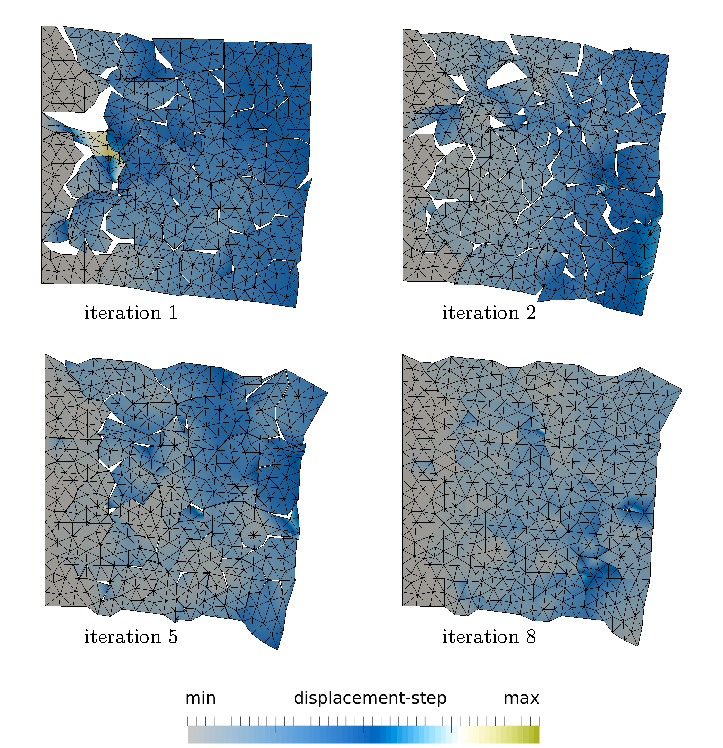
\includegraphics[width=0.7\textwidth]{./fig/tikz/study_contractfac_steps_visualization.pdf}
    \caption[Visualization of search directions in FETI-S]{Visualization of the search directions in an Simultaneous FETI simulation of the problem setup described in Figure~\ref{fig:setup_visualization_searchdirs}. All figures are warped by differently scaled displacement vectors for better visualization. The color corresponds to the step that the algorithm takes in that iteration. The figures show two things. Firstly, the algorithm is obviously very effective in capturing the largest errors. Secondly, with an increasing iteration number, the steps are effectively concentrated on very small areas. This is very well reflected in Figure~\ref{fig:results_study_contractfac}, where the number of search directions, that the FETI-AS solver chooses to work on, significantly reduces over the iterations and explains why FETI-AS shows hardly any slowdown in the convergence compared to FETI-S.}
    \label{fig:visualization_fetias_searchdirs}
  \end{center}
\end{figure}


\subsection{Fast Adaptive Simultaneous FETI(FETI-FAS)}\label{sec:fetifas}
The previous section has highlighted the potential superiority of the FETI-AS solver compared to the FETI-S one. Many search directions seem to be not that important, so neglecting them does not really increase the total iteration count much.\\
Looking at Figure~\ref{fig:results_study_contractfac} one can also note two things. Firstly, it seems that with progressing iteration, more and more search directions can be neglected, while it does make sense to use all search directions at first.\\
Secondly, the optimal choice of $\tau$ is crucial and, unfortunately, it is problem-dependent. This problem can be avoided by prescribing a contraction factor $\rho$ according to Equation~\eqref{eq:general_ampcg_conditions}, this does, however, introduce an eigenvalue problem and it is often difficult to draw a clear line between the smallest eigenvalue and eigenvalues that are numerically zero, due to the projection.\\
This section is thus dedicated to a thorough analysis of these mechanisms. Specifically, new approaches will be introduced for the selection of important search directions. Since they avoid the expensive $\tau$-test, they will be denoted as Fast Adaptive Simultaneous FETI schemes(FETI-FAS) in this thesis.\\
Numerical analysis will finally test their robustness and performance compared to FETI-AS and conclusions will be drawn in Chapter~\ref{cha:summary}.


\paragraph{The problem with FETI-1/FETI-2}
For the following considerations, the setup already described in Figure~\ref{fig:setup_visualization_searchdirs} will be discussed. Iteration numbers for this problem have already been provided in Figure~\ref{fig:resuts_study_contractfac}. It seems that the more the algorithm is shifted towards the classical FETI-1 approach, the more rapidly the total iteration count increases. Indeed, the same problem solved with FETI-1 takes 147 iterations.\\
To analyse this behaviour the development of the convergence indicator $\ids{t}$ for the substructures has been visualized in Figure~\ref{fig:ts_development}. It can bee seen, that FETI-S is much more capable of improving the substructure solutions uniformly, compared to FETI-1. The reason is, that in FETI-1, all substructure directions are simply summed up. So few contributions dominate the sum. More over, the same force value, relating to a Lagrange multiplier, is used for both sides of the interface in FETI-1, which can lead to significant errors.\\
Noting that the calculation of $\ids{t}$ does not introduce a significant overhead, one could think of several ways to improve the convergence:
\begin{enumerate}
  \item Build blocks of search directions according to their contribution factor
  \item Select search directions which showed a decreasing contribution factor
  \item Select the search directions with lowest $\ids{t}$
\end{enumerate}


\begin{figure}[h!]
  \begin{center}
    \subimport{./}{\tikzpath/algorithm_fetifas_scheme1}
    \caption[Structogram FETI-FAS scheme 1]{Scheme 1 for the FETI-FAS approach as described in Section~\ref{sec:fetifas}. The substructure convergence indicator as sorted in ascending order in each iteration. The substructure indices are then grouped block-wise, according to their convergence indicator. Each block gives one summed up search direction. The search space is then created with these search directions.}
    \label{strukt:fetifas_scheme1}
  \end{center}
\end{figure}

\begin{figure}[h!]
  \begin{center}
    \subimport{./}{\tikzpath/algorithm_fetifas_scheme2}
    \caption[Structogram FETI-FAS scheme 1]{Scheme 2 for the FETI-FAS approach as described in Section~\ref{sec:fetifas}. The substructure convergence factors are compared to the previous iterations. If it decreased than the search directions is incorporated into the search space. For a specified number of iterations at the beginning, all search directions are used. In order to avoid the incorporation of search directions that relate to already converged substructures due to numerical fluctuations, search directions are no longer incorporated into the search space, if their convergence factor has converged up to a factor of 100 to the simulation tolerance. For all calculations during this thesis, this barrier has shown to be practical.}
    \label{strukt:fetifas_scheme1}
  \end{center}
\end{figure}

\begin{figure}[h!]
  \begin{center}
    \subimport{./}{\tikzpath/algorithm_fetifas_scheme3}
    \caption[Structogram FETI-FAS scheme 1]{Scheme 3 for the FETI-FAS approach as described in Section~\ref{sec:fetifas}. The substructure convergence indicator as sorted in ascending order in each iteration. Only the directions with lowest $t_i^s$ are incorporated into the search space.}
    \label{strukt:fetifas_scheme1}
  \end{center}
\end{figure}

The results for all three approaches are visualized in Figure~\ref{fig:fetifas_schemes}. Due to the results of that figure, scheme 2 has been favoured for the rest of this thesis. If not mentioned otherwise FETI-FAS refers to that scheme from now on

\begin{figure}[h!]
  \begin{center}
    \includestandalone{\tikzpath/study_contractfac_ts-development}
    %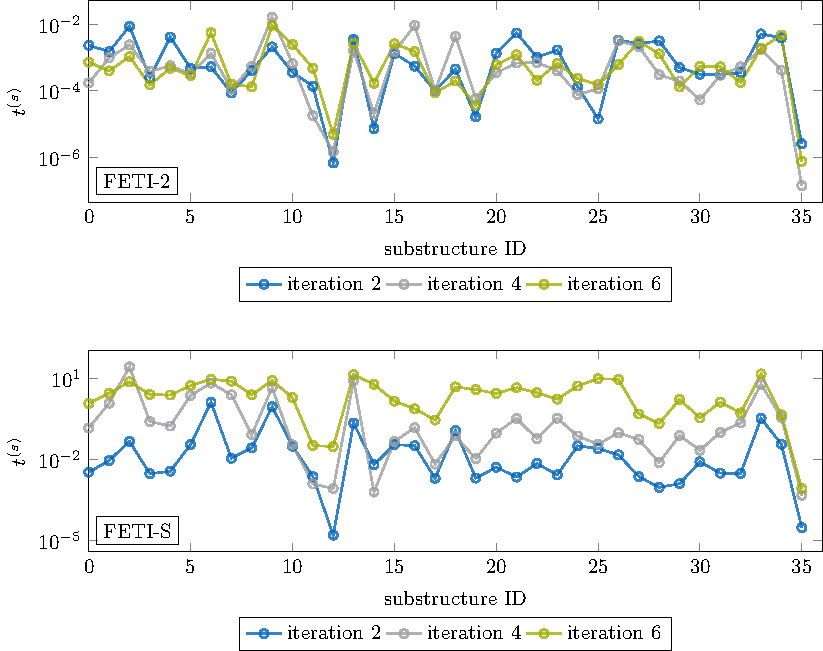
\includegraphics[width=\textwidth]{./fig/tikz/study_contractfac_ts-development.pdf}
    \caption[Development of convergence indicator during FETI-2 and FETI-S iterations]{Plot of the substructure convergence indicator $\ids{t}$ for FETI-2 and FETI-S. Of course, $\ids{t}$ is irrelevant for those solvers. However, they give a pretty good interpretation on how the choice of $\tau$ influences the converge properties of a FETI-AS simulations. Every FETI-AS search space includes the direction, created by the simple sum of preconditioners, as can be seen in Figure~\ref{strukt:fetias}. Some directions are then additionally added according to the so called $\tau$-test(step (15) in Figure~\ref{strukt:fetias}). If all directions are added, a classical FETI-S is retrieved.}
    \label{fig:ts_development}
  \end{center}
\end{figure}



\begin{figure}[h!]
  \begin{center}
    \includestandalone{\tikzpath/study_contractfac_fetifas}
    %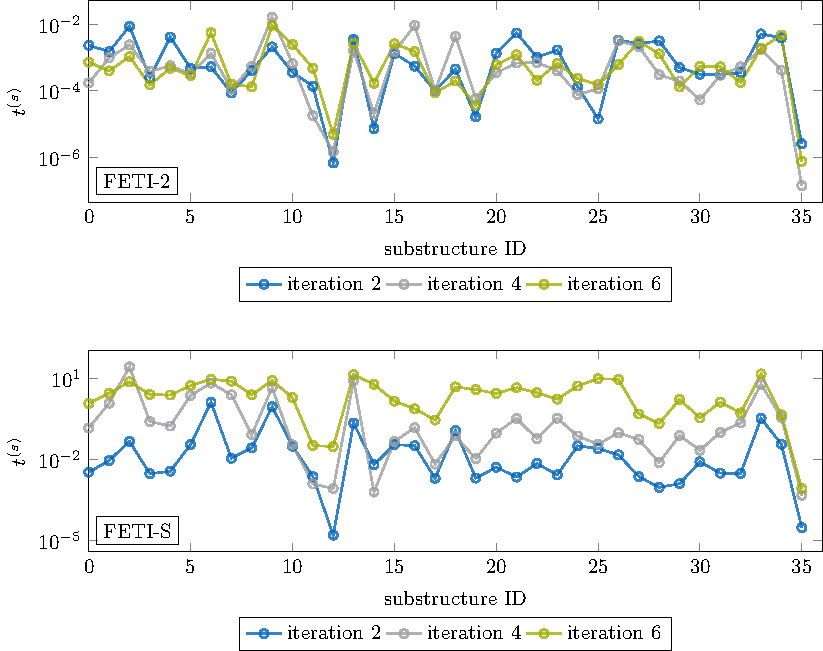
\includegraphics[width=\textwidth]{./fig/tikz/study_contractfac_ts-development.pdf}
    \caption[Results for the proposed FETI-FAS schemes]{For scheme 1 two search directions, built by the sum of the the lower and upper half of search directions sorted by $t_s^i$ respectively, were used. Scheme 2 was implemented just as described in Section~\ref{sec:fetifas}.For scheme 3, the four search directions with lowest $\ids{t}$ have been used in each iteration. }
    \label{fig:fetifas_schemes}
  \end{center}
\end{figure}






%\section{FETI-B}
%The block FETI method (FETI-B) is based on the idea of the block Conjugate Gradient algorithm~\cite{OLeary1980}.
%Compared to FETI-1, a block of right hand sides is used to activate the local effects. In other words, it exploits the additive structure of the interface displacements $\ifacedispvec$ just like FETI-S exploits the additive structure of the pre-conditioner. The FETI-B method was first proposed in~\cite{Gosselet2015}, and has shown to require slightly less iterations than the FETI-S method. However it introduces the drawback of additional local Dirichlet and Neumann solves, while the main advantage, the elimination of full re-orthogonalization, can not be exploited in real codes, due to round-off error.\\
%First numerical studies, however, have attested the method noticeable reductions in the iteration numbers when it comes to cross-points and very irregular meshes. The method, however, still requires further investigation.\\
%A detailed explanation of the FETI-B algorithm is provided in Figure~TODO

\chapter{Numerical Assessment}\label{cha:numerical_assesment}
The previous chapter has introduced the FETI method as an efficient implementation of the domain decomposition approach for the purpose of parallelization. However, as any DD method, FETI struggles with some conditioning problems, especially as the number of sub-domains increases.\\
Chapter \ref{cha:feti_solvers} introduced several variations of the original FETI-method. Some of which were derived exactly for the purpose of handling the numerical difficulties. Since all mentioned methods have been implemented into the FEMAC code\cite{FEMAC}, the following chapter provides a profound numerical analysis of the presented methods and their capabilities to handle the heterogeneities along and across the interface, different partitioning schemes, irregular interfaces, incompressibility and inclusion problems. Taking into account the computational effort and scalability issues, conclusions will be drawn, and recommendations will be provided in Chapter~\ref{cha:summary}.
\\
\section{Default parameters}\label{sec:default_parameters}
The previous chapter have already introduced numerous parameters and choices to be made for the FETI solvers. If not explicitly specified otherwise, the following parameters have been used for all calculations in this thesis.
\\
\begin{center}
  \begin{tabular}{|l|l|}
    \hline
    \textbf{Termination criterion} &Residual of $10^{-6}$ \\
    \hline
    \textbf{Preconditioner type}   & Lumped                                               \\
    \hline
    \textbf{A-matrix}              & Unity matrix                                         \\
    \hline
    \textbf{Scaling}               & Multiplicity scaling                                 + K-scaling \\
    \hline
    \textbf{$\rho$ for FETI-AS}    & $0.999$                                               \\
    \hline
    \textbf{FETI-2 coarse grid}    & Geneo with 6 lowest eigenmodes per substructure                            \\
    \hline
  \end{tabular}
\end{center}


\section{Conditioning}\label{sec:condnum}

As explained in Chapter~\ref{cha:introduction}, the FETI type of solvers are hybrids between direct and iterative solvers. A large problem is typically divided into a number of substructures large enough such that each sub-problem can be solved for directly in reasonable time. The hybridization is introduced in the formulation when it comes to solving the connecting interface problem. As explained in Section~\ref{sec:iterative_theory} and outlined algorithmically in Section~\ref{sec:cg}, iterative methods like the Conjugate Gradient algorithm are typically used for this purpose.\\
As any iterative method, a CG algorithm is quite susceptible to bad condition numbers. It should be noted at this point, that the conditioning is a property of the problem formulation, not the algorithm itself. Of course, the absolute value of $\condnum$ depends on the norm used, it should therefore be used only for relative statements.\\

\subsection{Theory}
We consider a linear system of equations
\begin{align}
  \dmat{A} \dvec{x} = \dvec{b} 
\end{align}
We know, that if $det(\dmat{A})=0$, in other words A is singular, this system does not have a solution.\\
If, on the other hand, $det(\dmat{A})\neq 0$, the convergence of an iterative scheme is determined by the condition number defined as $\condnum=\norm{\dmat{A}} \norm{\inv{\dmat{A}}} $.\\
Every iterative algorithm basically works by creating an update on the current solution by considering the residual defined as
\begin{align}
  \dvec{r}^{k}=\dvec{b}-\dmat{A} \dvec{x}^{k} 
\end{align}
The accuracy of the solution is usually defined in terms of the residual as
\begin{align}
  \epsilon=\norm{\dvec{r}}=\norm{\dvec{b}-\dmat{A} \dvec{x}^{k}} 
\end{align}
\\
It his well known that the error will decrease at minimum by a factor of $2 \left( \frac{\sqrt{\condnum}-1}{\sqrt{\condnum}+1} \right)^{i}$ in $k$ steps.


\subsection{Conditioning of the FETI problem}

The previous section indicated, that the condition number of the linear system solved plays a crucial role for the convergence properties of the FETI solver. In fact, some variations like the FETI-Geneo approach explicitly exploit that knowledge by removing "bad components" from the iteration space with the goal of improving the condition number. This chapter will introduce several vivid problem setups that lead to badly conditioned operators. One major challenge are heterogeneities of the material properties along, or across the interface.\\
From an engineering point of view, challenges tend to arise, when the behaviour of a substructure on its own, differs strongly from its behaviour when embedded into the whole system.\\
Figure~\ref{fig:setup_heterogenities_along_interface} introduces a standard DD problem setup. It consists of a sandwich-structure-like material distribution that resembles real life composite materials. The beam is divided into 16 regular substructures along the x-axis and is subjected to a load on the right face, while mounted in a statically determined manner on the left. The setup was solved with different FETI solvers and the eigenvalue distribution of the iteration matrix analysed in Figures~\ref{fig:eigvalues_pointdistribution} and~\ref{fig:eigvalues_histograms}.

\begin{figure}[tb]
  \begin{center}
    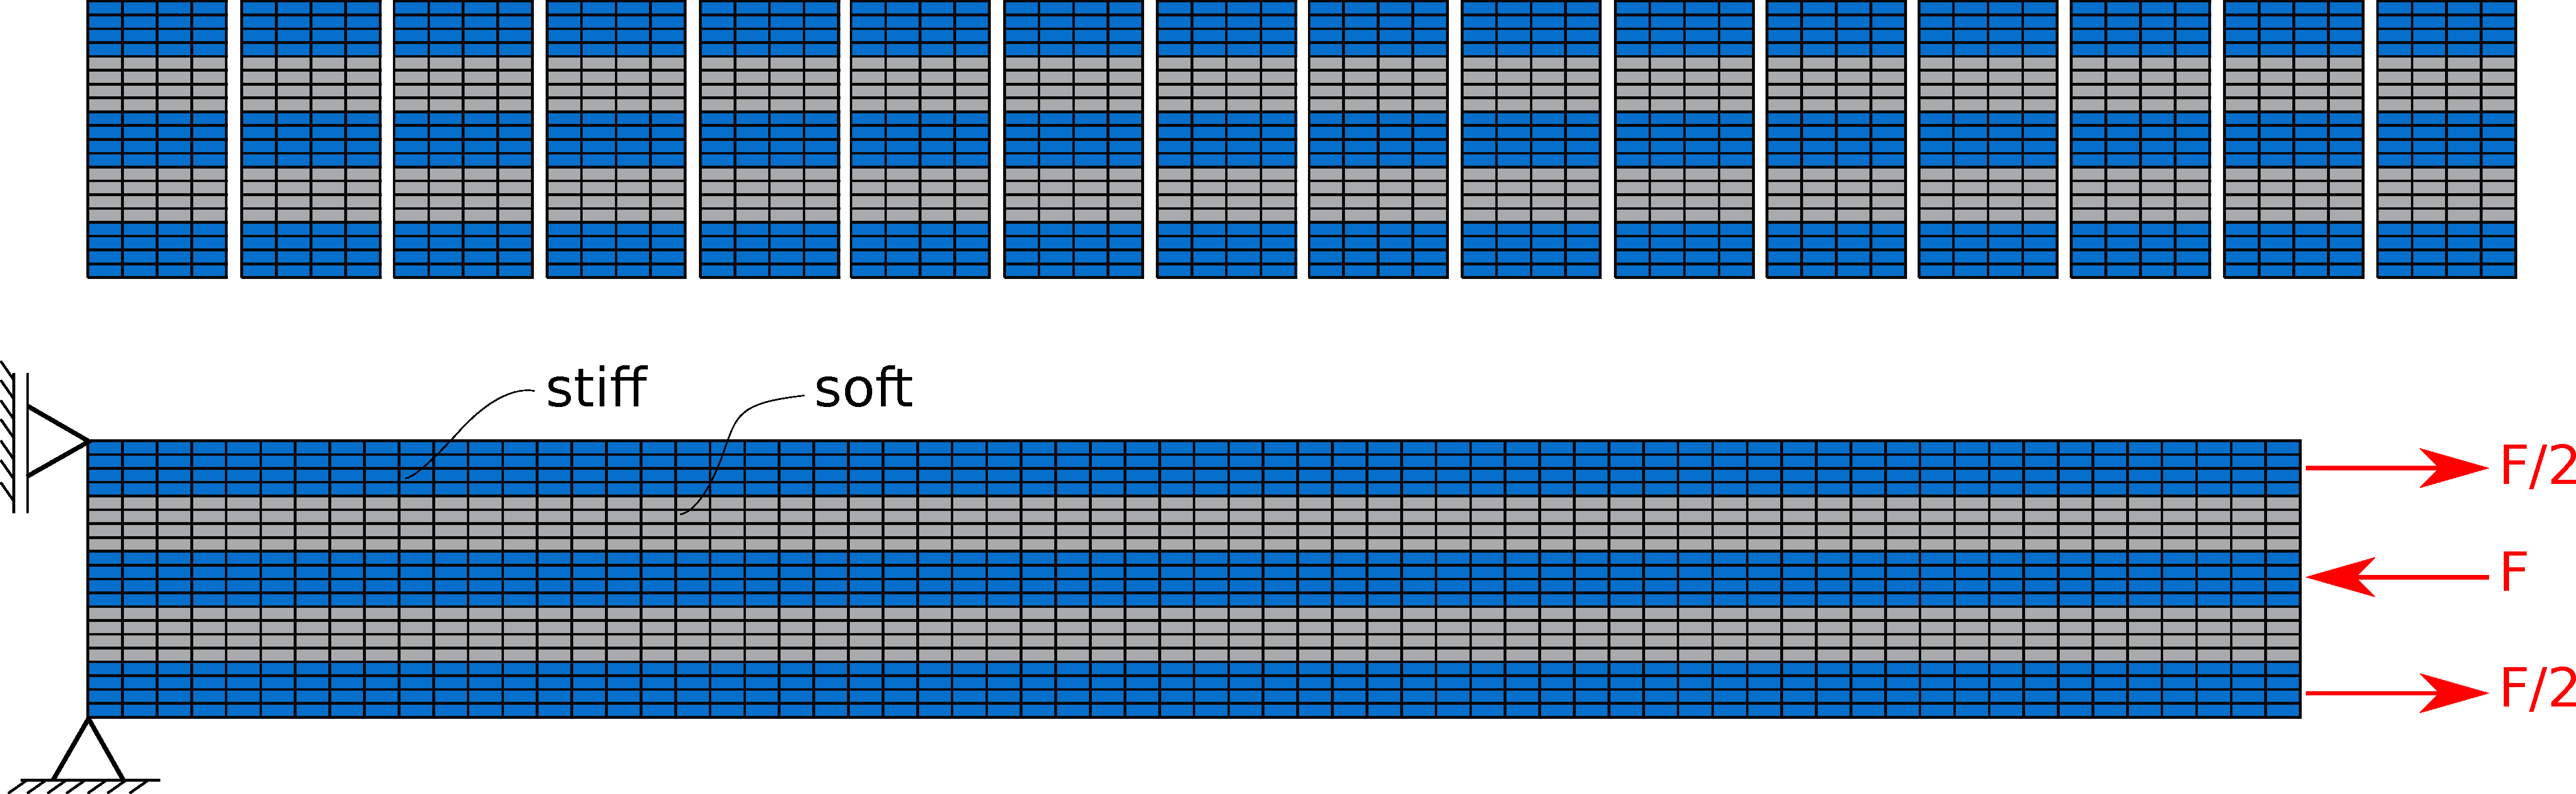
\includegraphics[width=0.8\textwidth]{\studypath/2016-08-18_EigenvalueDistribution/setup/setup_materials_partitions.pdf}
    \caption[Study of eigenvalue distribution: setup]{Setup for the eigenvalue analysis regarding heterogeneities along the interface. Note that the forces in this example are self-equilibrated, thus the solution does not contain rigid body modes. For the FETI-1 solver, rigid body components are the only information that is propagated globally. Therefore, calculating this special example leads to the phenomenon depicted in Figure~\ref{fig:beam_error_propagation}. The information can only travel one substructure after another during the iterations. The lack of means to transport non rigid-body mode errors globally is one reason, why the FETI-1 algorithm often shows very high iteration counts.}
    \label{fig:setup_heterogenities_along_interface}
  \end{center}
\end{figure}


\begin{figure}[tb]
  \begin{center}
    %\fbox{\subimport{./}{./fig/tikz/study_inclusion.tex}}
    \includestandalone{./fig/tikz/study_eigvalues_pointdistribution}
    \caption[Study of eigenvalue distribution: distributions]{The figures show the eigenvalues of the dual schur operator $\locdualschur$ for the different solver types. The top left figure shows the unprojected, unpreconditioned operator. Obviously, the eigenvalue distribution is pretty bad which would, as explained in Section~\ref{sec:ppcg}, drastically deteriorate performance. The bottom figure thus shows the dual schur operator after projection to the natural subspace(FETI-1) as well as after the projection into the auxiliary coarse space(FETI-2(GENEO)). Obviously, the projectors catch the extreme, isolated eigenvalues very well. Since the out-projected modes, that are related to the numerically zero eigenvalues in the middle figure have no influence on the following CG algorithm, they have been dropped in the bottom left figure, for better visualization.\\
    Finally, the bottom figure shows the comparison of the unprojected, unpreconditioned CG with the fully projected ones. Obviously, the condition number has been improved by several orders of magnitudes.}
    \label{fig:eigvalues_pointdistribution}
  \end{center}
\end{figure}

\begin{figure}[tb]
  \begin{center}
    %\fbox{\subimport{./}{./fig/tikz/study_inclusion.tex}}
    \includestandalone{./fig/tikz/study_eigvalues_histograms}
    \caption[Study of eigenvalue distribution: histograms]{The figure shows the eigenvalues of the  raw operator $\dmat{A}$(top left picture), the preconditioned operator $\dmat{H}\dmat{A}$(top right picture), the projected preconditioned operator as in FETI-1 $\dmat{H}\dmat{A}\dmat{\Pi}$(bottom left picture) and the 2-level projected, preconditioned operator as in FETI-2 $\dmat{H}\dmat{A}\dmat{\Pi}\dmat{\Pi_c}$(bottom right figure), as described in Chapter~\ref{cha:iterative_solvers}. One clearly sees, that the Projectors do catch bad modes very successfully, thus the condition number is improved.}		\label{fig:eigvalues_histograms}
  \end{center}
\end{figure}~

\begin{figure}[tb]
  \begin{center}
    %\subimport{./}{./fig/tikz/beam_error_progpagation_feti1}
    \includestandalone[subpreambles=true]{./fig/tikz/beam_error_progpagation_feti1}
    \caption[Limited error propagation FETI-1]{Visualization of the error propagation in FETI-1 for the setup described in Figure~\ref{fig:setup_heterogenities_along_interface}. It can be seen quite clearly, that the error propagation is limited to neighbouring substructures from one iteration to the other. The introduction of an auxiliary coarse grid solves this problem by introducing a mean of propagating the error globally. This example is particularly bad, since the forces are self equilibrated. Thus, FETI-1 has no means of propagating the error globally. For this reasons, information passes only one substructure at a time, which leads to very high iteration numbers for an increasing number of subdomains. }
    \label{fig:beam_error_propagation}
  \end{center}
\end{figure}

\section{Heterogeneities}\label{sec:heterogeneities}
One of the most challenging problems for domain decomposition methods are changing constitutive parameters(material heterogeneities) along, as well across the interface. The reason for this has been explained in Section~\ref{sec:condnum}.\\
From an engineering point of view, problems always occur if substructures on their own show a very different behaviour as compared to them being embedded in the total system. Algorithmically, it does make a large difference whether heterogeneities are along or across the interface. This section therefore is denoted to an extensive analysis of the proposed FETI Solvers with regards to the two types. The material patterns used for this study are provided in Figure~\ref{fig:heterogenity_materials_patterns}.


\begin{figure}[tb]
  \begin{center}
    \begin{subfigure}[b]{\textwidth}
      \centering
      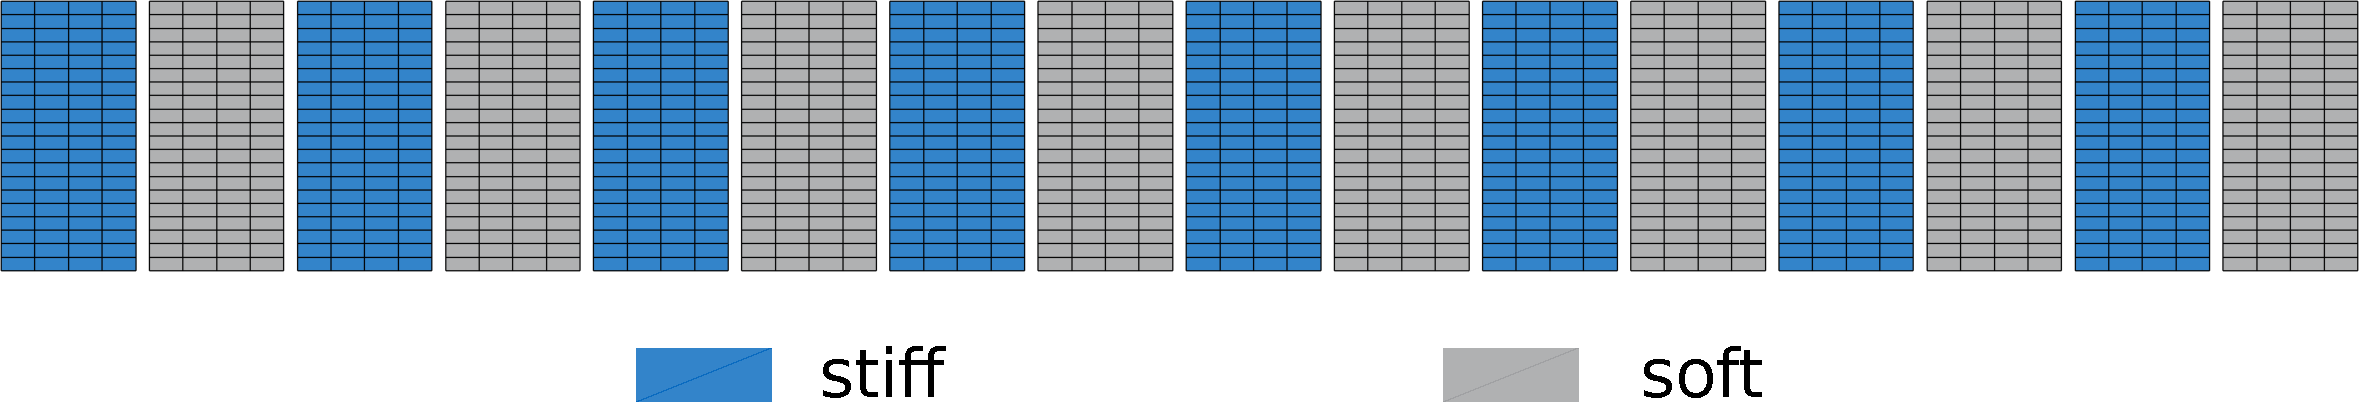
\includegraphics[width=0.6\textwidth]{\studypath/2016-08-22_HeterogenityType/setup/materials_vertical.pdf}
      \caption{Heterogeneities across the interface}
    \end{subfigure}
    \vskip\baselineskip
    \begin{subfigure}[b]{\textwidth}
      \centering
      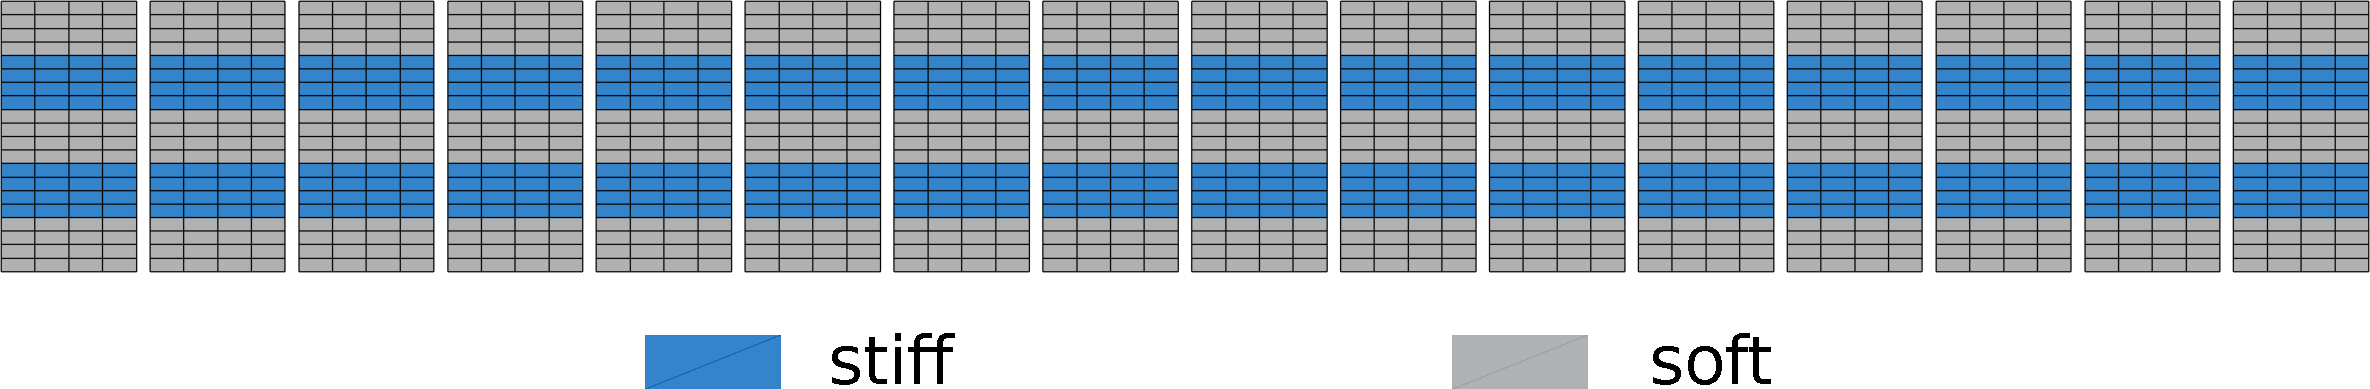
\includegraphics[width=0.6\textwidth]{\studypath/2016-08-22_HeterogenityType/setup/materials_horizontal.pdf}
      \caption{Heterogeneities along the interface}
    \end{subfigure}
    \vskip\baselineskip
    \begin{subfigure}[b]{\textwidth}
      \centering
      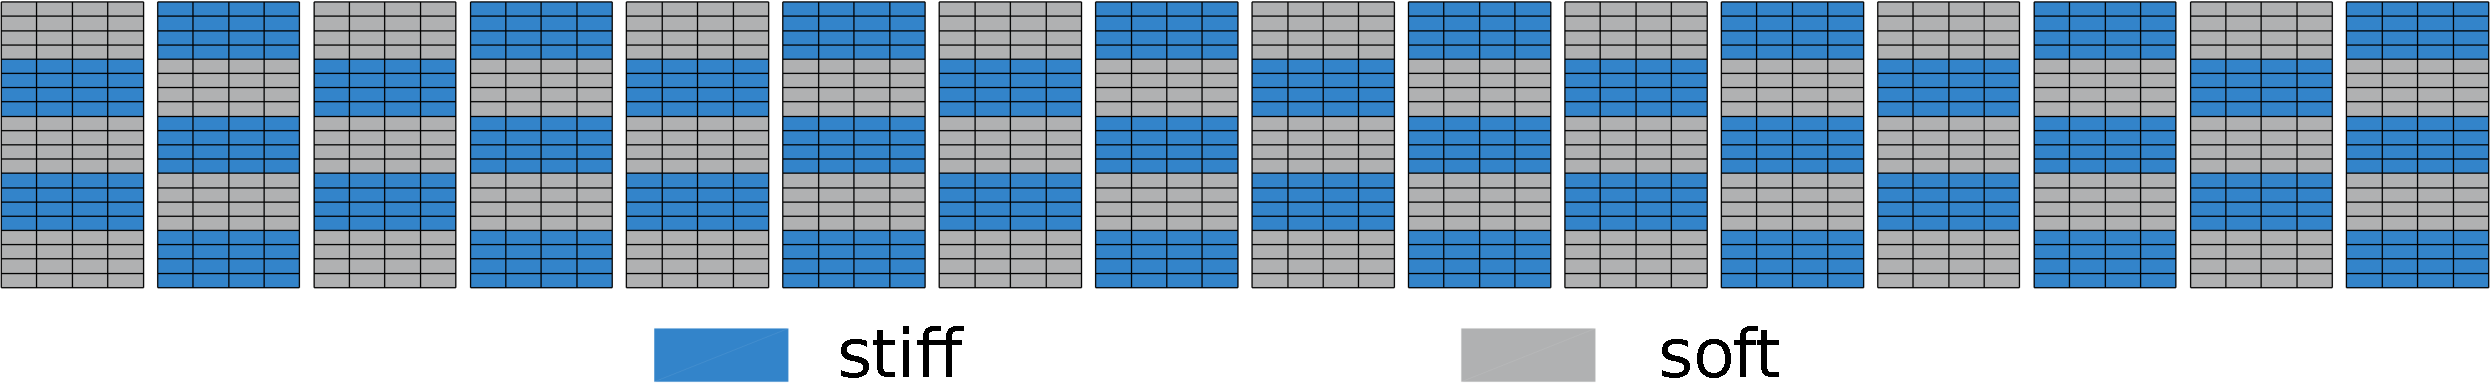
\includegraphics[width=0.6\textwidth]{\studypath/2016-08-22_HeterogenityType/setup/materials_checkerboard.pdf}
      \caption{Combined heterogeneities}
    \end{subfigure}
    \caption[Study of heterogeneities: material patterns]{Material patterns for the heterogeneity analysis. The substructuring has been done such, that the setup at the top shows heterogenities only across the interface and the middle one only along the interface. The checkerboard pattern at the bottom shows both, heterogeneities across and along the interface. The beams were clamped on the left side and subjected to a uniform downward force on the right.}
    \label{fig:heterogenity_materials_patterns}
  \end{center}
\end{figure}



\subsection{Heterogeneities across the interface}\label{sec:heterogeneities_across}
A typical example of heterogenities across the interface is described in the top of Figure~\ref{fig:heterogenity_materials_patterns}. The beam is clamped on the left face and subjected to a uniform downward force on the right face\\
The reason for the problems with this type of heterogeneity have been explained in Section~\ref{sec:precond}.\\
During the FETI iterations, intermediate solutions for the interface forces are found. Based on this force, a resulting displacement is predicted. In a standard, non scaled FETI-algorithm, this displacement is then applied in equal parts on the two substructure interfaces concerned. If now the substructure on one side of the interface is significantly stiffer, than the other one, this simple 50/50 approach, of course, leads to very wrong results. A possible solution to this problem is K-scaling, which has been derived in \cite{Farhat1995}. If not mentioned otherwise, this code does always use k-scaling and multiplicity scaling as explained in Section~\ref{sec:precond}.\\
The problem of heterogenities across the interface is visualized in Figure~\ref{fig:study_heterogeneity_results_across}.

\begin{figure}[tb]
  \begin{center}
    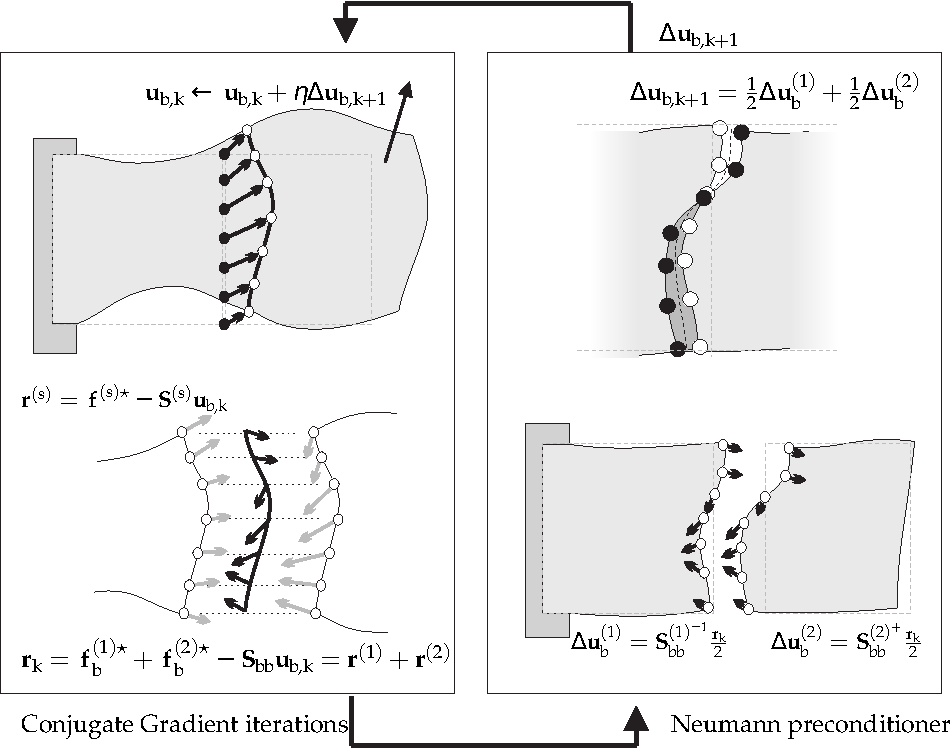
\includegraphics[width=0.5\textwidth]{./fig/pdf/problem_heterogenity.pdf}
    \caption[Study of heterogeneities across the interface: problem sketch]{Sketch of the Problem related to heterogenities across the interface. The figure was taken from~\cite{Rixen2013}. Through the simple sum of contributions in the preconditioner, all substructures contribute equally to the search direction. The Neumann step thus equally displaces both interface sides. If, however, one side of the interface shows a much higher stiffness than the other, the natural solution would actually be such, that the soft material shows a much higher displacement than the stiff one. If this discrepancy is not dealt with, convergence rates can be severely damaged. One possible solution would be K-scaling, as described in~\cite{Rixen1999a}. Also, thanks to its independent substructure-based search directions, FETI-S is not that susceptible to this problem.}
    \label{fig:problem_heterogenity_sketch}
  \end{center}
\end{figure}



\begin{figure}[tb]
  \begin{center}
    %\fbox{\subimport{./}{./fig/tikz/study_inclusion.tex}}
    \includestandalone{./fig/tikz/study_heterogenity_vstripes}
    \caption[Study of heterogeneities across the interface: \# iterations]{Results for the convergence analysis of the FETI algorithms for materials across the interface. The left figure shows the results without scaling, the left figure shows the results with scaling. The graphs do show two things. First of all, the multi preconditioned schemes seem to be far less effected by this type of heterogeneity, that the singe preconditioned ones.  Secondly, the scaling is very effective in reducing the iteration numbers for FETI-1. It also seems that K-scaling is mandatory for the FETI-2(Geneo) approach to work properly here. Since the numerical effort is low, it is therefore always recommended to use a k-scaling when high heterogeneities are present.}
    \label{fig:study_heterogeneity_results_across}
  \end{center}
\end{figure}

\begin{figure}
  \begin{center}
    \includestandalone{./fig/tikz/study_heterogenity_vstripes_residual}
    \caption[Study of heterogeneities across the interface: residua]{Residuum development for the convergence analysis of the FETI algorithms regarding heterogeneities across the interface, as described in the top of Figure~\ref{fig:heterogenity_materials_patterns}. Obviously K-scaling drastically improves performance here. The right figure shows that a PCG method(FETI-2) is capable of showing the same convergence rates as an MPCG one(FETI-S) provided that K-scaling is used. In that case, the reduced number of iterations of the FETI-S solver can be attributed to the reduced problem size solemnly. Finally, FETI-S seems to not have benefited much from the Scaling approach. This seems reasonable since substructures interfaces are optimized independently of one another anyway}
    \label{fig:heterogeneity_accross_residuum}
  \end{center}
\end{figure}

\begin{figure}
  \begin{center}
    \includestandalone{./fig/tikz/study_heterogenity_vstripes_adaptive}
    \caption[Study of heterogeneities across the interface: \# search directions]{Results for the convergence analysis of the FETI algorithms for materials across the interface, as depicted at the top of Figure~\ref{fig:heterogenity_materials_patterns}. This figure show the number of search directions used by the different adaptive schemes. Overall, FETI-AS shows superior results here. What is more, K-scaling seems to completely eliminate the problems of heterogeneities across the interface, since in that case, no difference can be observed between a stiffness ratio of 10 and a ratio of 1000.}
    \label{fig:heterogeneity_accross_numsdir}
  \end{center}
\end{figure}









\FloatBarrier
\subsection{Heterogeneities along the interface}\label{sec:heterogeneities_along}
Heterogeneities along the interface are somewhat more difficult. The ill-conditioning can not be coped with by simple scaling methods. The material distribution used for this analysis is provided in Figure~\ref{fig:heterogenity_materials_patterns}. Iteration numbers are provided in Figure~\ref{fig:study_heterogeneity_results_along}, residua development in Figure~\ref{fig:heterogeneity_along_residuum} and a visualization of the number of used search directions in Figure~\ref{fig:heterogeneity_along_numsdir}.
%%%\begin{figure}[tb]
%%%	\begin{center}
%%%	    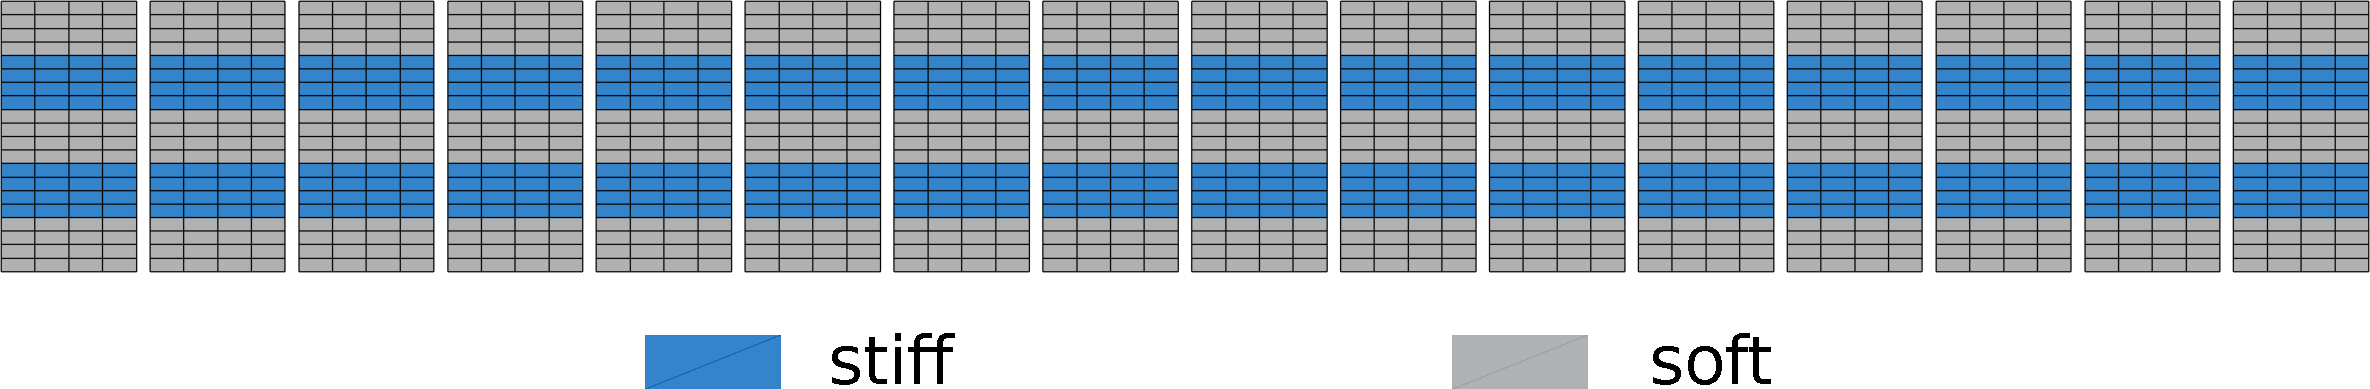
\includegraphics[width=0.5\textwidth]{\studypath/2016-08-22_HeterogenityType/setup/materials_horizontal.pdf}
%%%        \caption[Setup heterogeneity along interface]{Setup for the convergence analysis of the FETI algorithms with regards to heterogenities along the interface. The bearing of and the forces applied on the beam as well as its partitioning into substructures are visualized in Figure~\ref{fig:study_heterogenity_setup_bc}.}
%%%		\label{fig:study_heterogeneity_setup_along}
%%%    \end{center}
%%%\end{figure}

\begin{figure}[tb]
  \begin{center}
    %\fbox{\subimport{./}{./fig/tikz/study_inclusion.tex}}
    \includestandalone{./fig/tikz/study_heterogenity_hstripes}
    \caption[Study of heterogeneities along the interface: \# iterations]{Results for the convergence analysis of the FETI algorithms for materials along the interface. Again, FETI-2 shows severe problems. As expected, scaling does not improve the iteration counts significantly, since it is not designed to cope with this kind of heterogeneity. The multi preconditioned algorithms seem to be able to cope with the problem quite well. In contrast to the heterogeneities across the interface from Figure~\ref{fig:study_heterogeneity_results_across}, Geneo is capable of effectively detecting the bad modes and iteration counts can therefore be kept low successfully with FETI-2.}
    \label{fig:study_heterogeneity_results_along}
  \end{center}
\end{figure}

\begin{figure}
  \begin{center}
    \includestandalone{./fig/tikz/study_heterogenity_hstripes_residual}
    \caption[Study of heterogeneities along the interface: residua]{Residuum development for the convergence analysis of the FETI algorithms regarding heterogeneities along the interface, as described at the middle of Figure~\ref{fig:heterogenity_materials_patterns}. Obviously, K-scaling does not effect the convergence properties at all. What is more, MPCG methods show significantly better results than the PCG ones. In particular, Geneo performed much worse than for the case of heterogeneities across the interface. It remains to be analysed whether a larger coarse space would improve its properties, but, as explained earlier, increasing the coarse problem has significant drawbacks. }
    \label{fig:heterogeneity_along_residuum}
  \end{center}
\end{figure}

\begin{figure}
  \begin{center}
    \includestandalone{./fig/tikz/study_heterogenity_hstripes_adaptive}
    \caption[Study of heterogeneities across the interface: \# search directions]{Results for the convergence analysis of the FETI algorithms for materials along the interface, as described at the middle of Figure~\ref{fig:heterogenity_materials_patterns}. This figures visualizes the number of search directions used by the multi preconditioned schemes during the iterations. At least for the contraction factor of 0.999, the overall improvement is not satisfactory. FETI-AS, however still gives quite nice results with the standard parameters as defined in Section~\ref{sec:fetias}. }
    \label{fig:heterogeneity_along_numsdir}
  \end{center}
\end{figure}





\FloatBarrier
\subsection{Combined heterogeneities}\label{sec:heterogeneities_combined}
In real engineering problems, especially when automatic graph partitioners like Metis are used, one will most likely have to deal with a combined form of heterogeneity. Therefore a setup that contains both shall now be considered. The material pattern is depicted in the bottom of Figure~\ref{fig:heterogenity_materials_patterns}. Iteration numbers are provided in Figure~\ref{fig:study_heterogenity_combined}, numbers of used search directions in Figure~\ref{heterogeneity_combined_numsdir} and the residuum development in Figure~\ref{fig:heterogeneity_cboard_residuum}.


\begin{figure}[tb]
  \begin{center}
    %\fbox{\subimport{./}{./fig/tikz/study_inclusion.tex}}
    \includestandalone{./fig/tikz/study_heterogenity_cboard}
    \caption[Study of combined heterogeneities: \#iterations]{Results for the convergence analysis of the FETI algorithms for materials across and along the interface. As expected, FETI-1 performs very poorly. K-scaling does not really improved the iteration numbers, except for FETI-2, where we have already seen in Figure~\ref{fig:heterogeneity_along_numsdir} that it is not able to build an appropriate coarse grid for the case of heterogenities. As could be expected from Figures~\ref{fig:study_heterogeneity_results_across} and~\ref{fig:study_heterogeneity_results_along}, the multi-preconditioned algorithms show superior properties.}
    \label{fig:study_heterogenity_combined}
  \end{center}
\end{figure}

\begin{figure}
  \begin{center}
    \includestandalone{./fig/tikz/study_heterogenity_cboard_residual}
    \caption[Study of combined heterogeneities: residua]{Residuum development for the convergence analysis of the FETI algorithms regarding combined heterogeneities, as depicted at the bottom of Figure~\ref{fig:heterogenity_materials_patterns}. This figure shown the development of the residual over the iterations for al solvers. Obviously, K-scaling is not capable of significantly reducing the the total number of iterations, except for FETI-2(Geneo), where we have already observed that it seems to be necessary for the construction of an effective coarse space.}
    \label{fig:heterogeneity_cboard_residuum}
  \end{center}
\end{figure}

\begin{figure}
  \begin{center}
    \includestandalone{./fig/tikz/study_heterogenity_cboard_adaptive}
    \caption[Study of combined heterogeneities: \# search directions]{Results for the convergence analysis of the FETI algorithms regarding combined heterogeneities, as depicted at the middle of Figure~\ref{fig:heterogenity_materials_patterns}. This figure shows the number of search directions used by the multi preconditioned solvers for all iteration steps. Both FETI-AS ans FETI-FAS were capable of significantly reducing the total number of search directions used.}
    \label{heterogeneity_combined_numsdir}
  \end{center}
\end{figure}





\section{Partitioning}
For a domain decomposition method like FETI, the question of how to form the substructures comes naturally. Partitioning is typically done by automatic graph partitioning algorithms like Metis or Chaco. For some specific cases, however, it can be advantageous to choose partitions manually. Particularly, for the examples of a composite material, one can choose partitions such that the problems of heterogenities along the interface, as described in Section~\ref{sec:heterogeneities} are avoided.\\
Nonetheless, even automatic graph partitioners offer some parameters to choose from. This section is therefore denoted to an analysis of different partitioning approaches.
\\
Figure~\ref{fig:partitioning_schemes} shows the four different partitioning schemes considered. The plate is clamped on the left side and subjected to a uniform surface load in y-direction on the right face.
\\
The partitions have been chosen such, that the interface problem has roughly the same size on all four setups. We can note right at this point, that stripe-like partitioning like in the bottom two subfigures, is far less efficient when it comes to keeping the number of interface unknowns low. For an equally sized interface problem, the number of substructure is more than three times less than for the regular partitioning in the top-left figure, a potential weak-point when it comes to parallizability.\\
However, as~\cite{Farhat1991} writes, stripe-like partitioning may offer the advantage of a reduced interconnectivity in the substructure stiffness matrices, solving the local problems may becomes faster thus.
\\
The results of this analysis are presented in Figure~\ref{fig:study_partitioning_numiter}.



\begin{figure}[tbp]
  \centering
  \begin{subfigure}[b]{0.3\textwidth}
    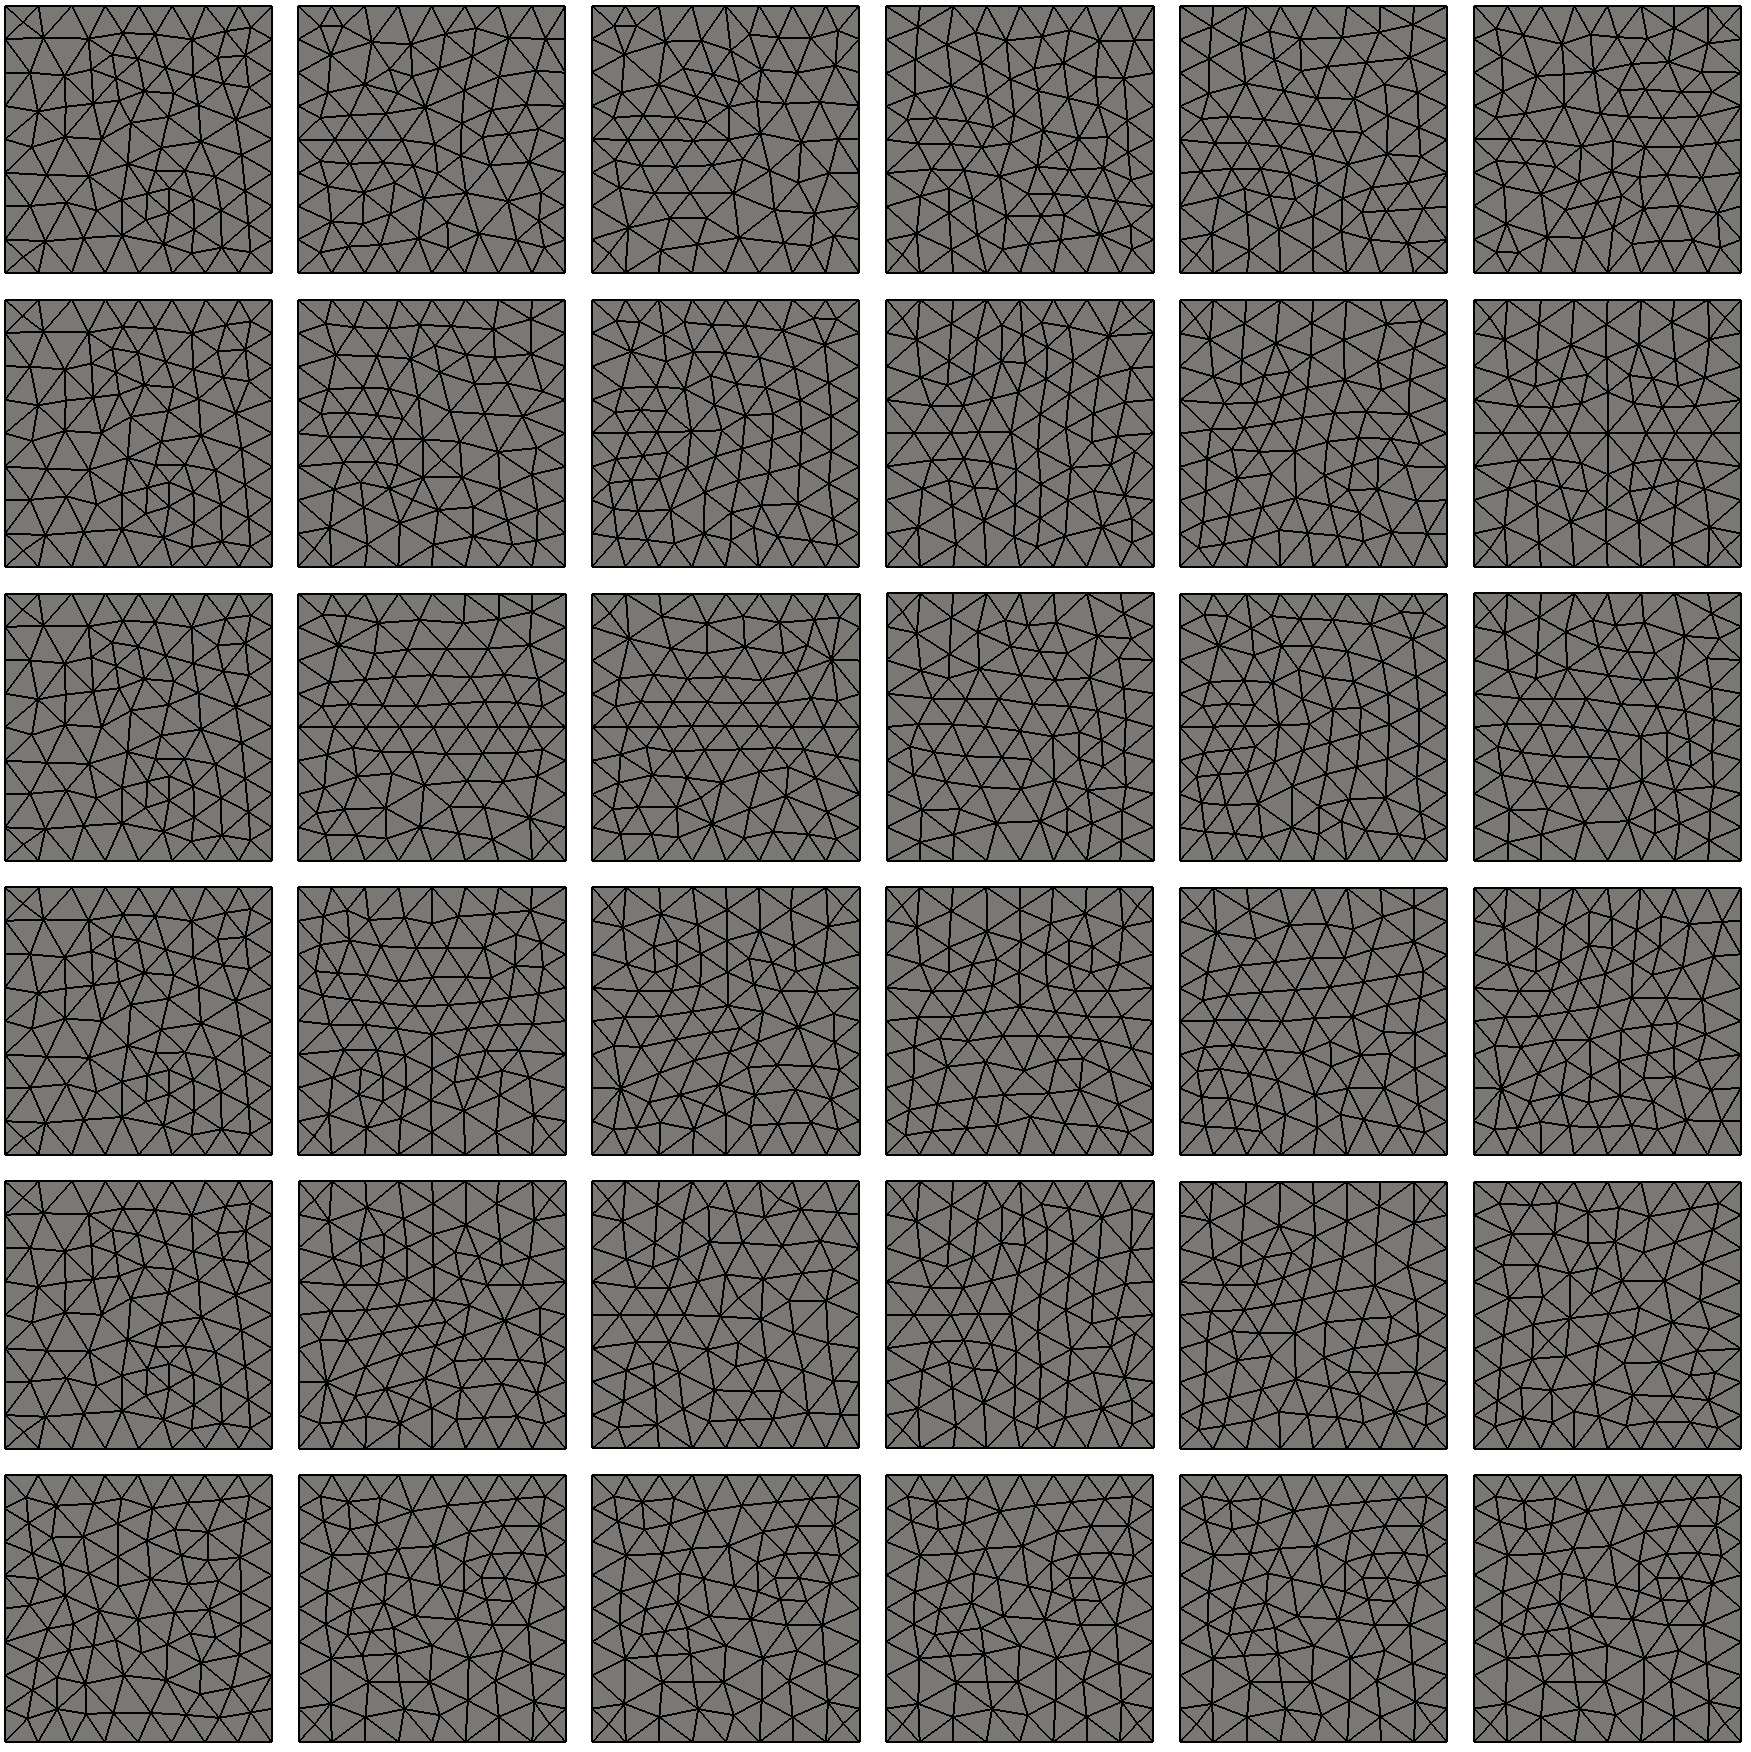
\includegraphics[width=\textwidth]{/home/lukas/Desktop/SA_Thesis/studies/2016-08-10_Partitioning/setup/regular_6x6.png}
    \caption{regular partitioning}
  \end{subfigure}
  \hspace{1cm}
  \begin{subfigure}[b]{0.3\textwidth}
    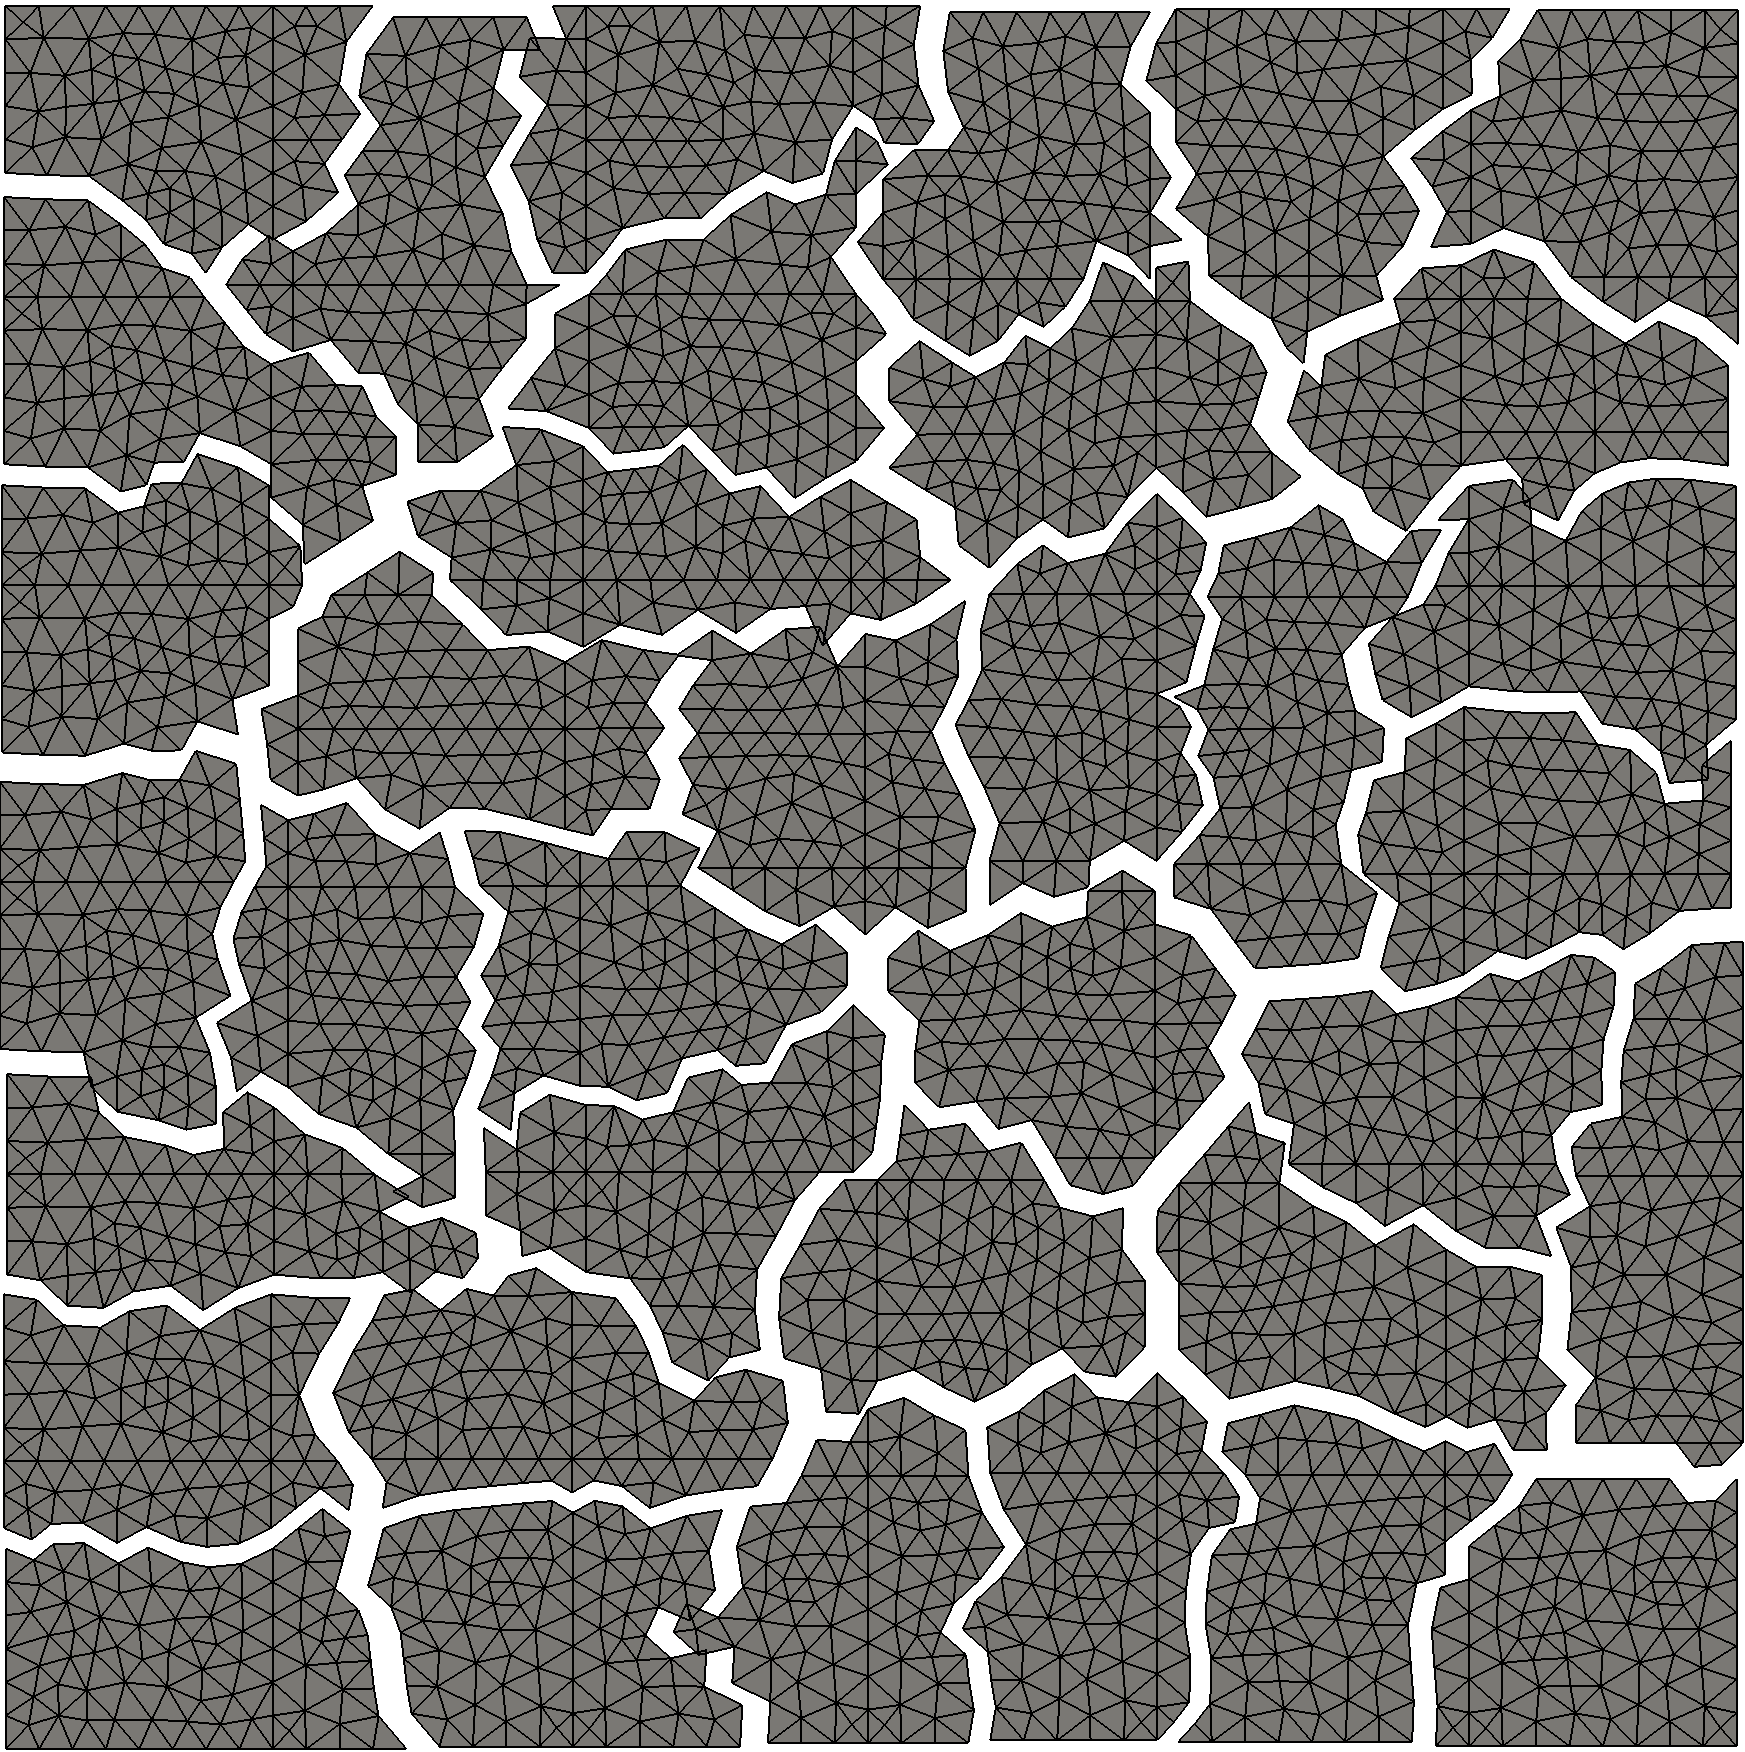
\includegraphics[width=\textwidth]{/home/lukas/Desktop/SA_Thesis/studies/2016-08-10_Partitioning/setup/chaco_6x6.png}
    \caption{automatic partitioning}
  \end{subfigure}
  \vskip\baselineskip
  \begin{subfigure}[b]{0.3\textwidth}
    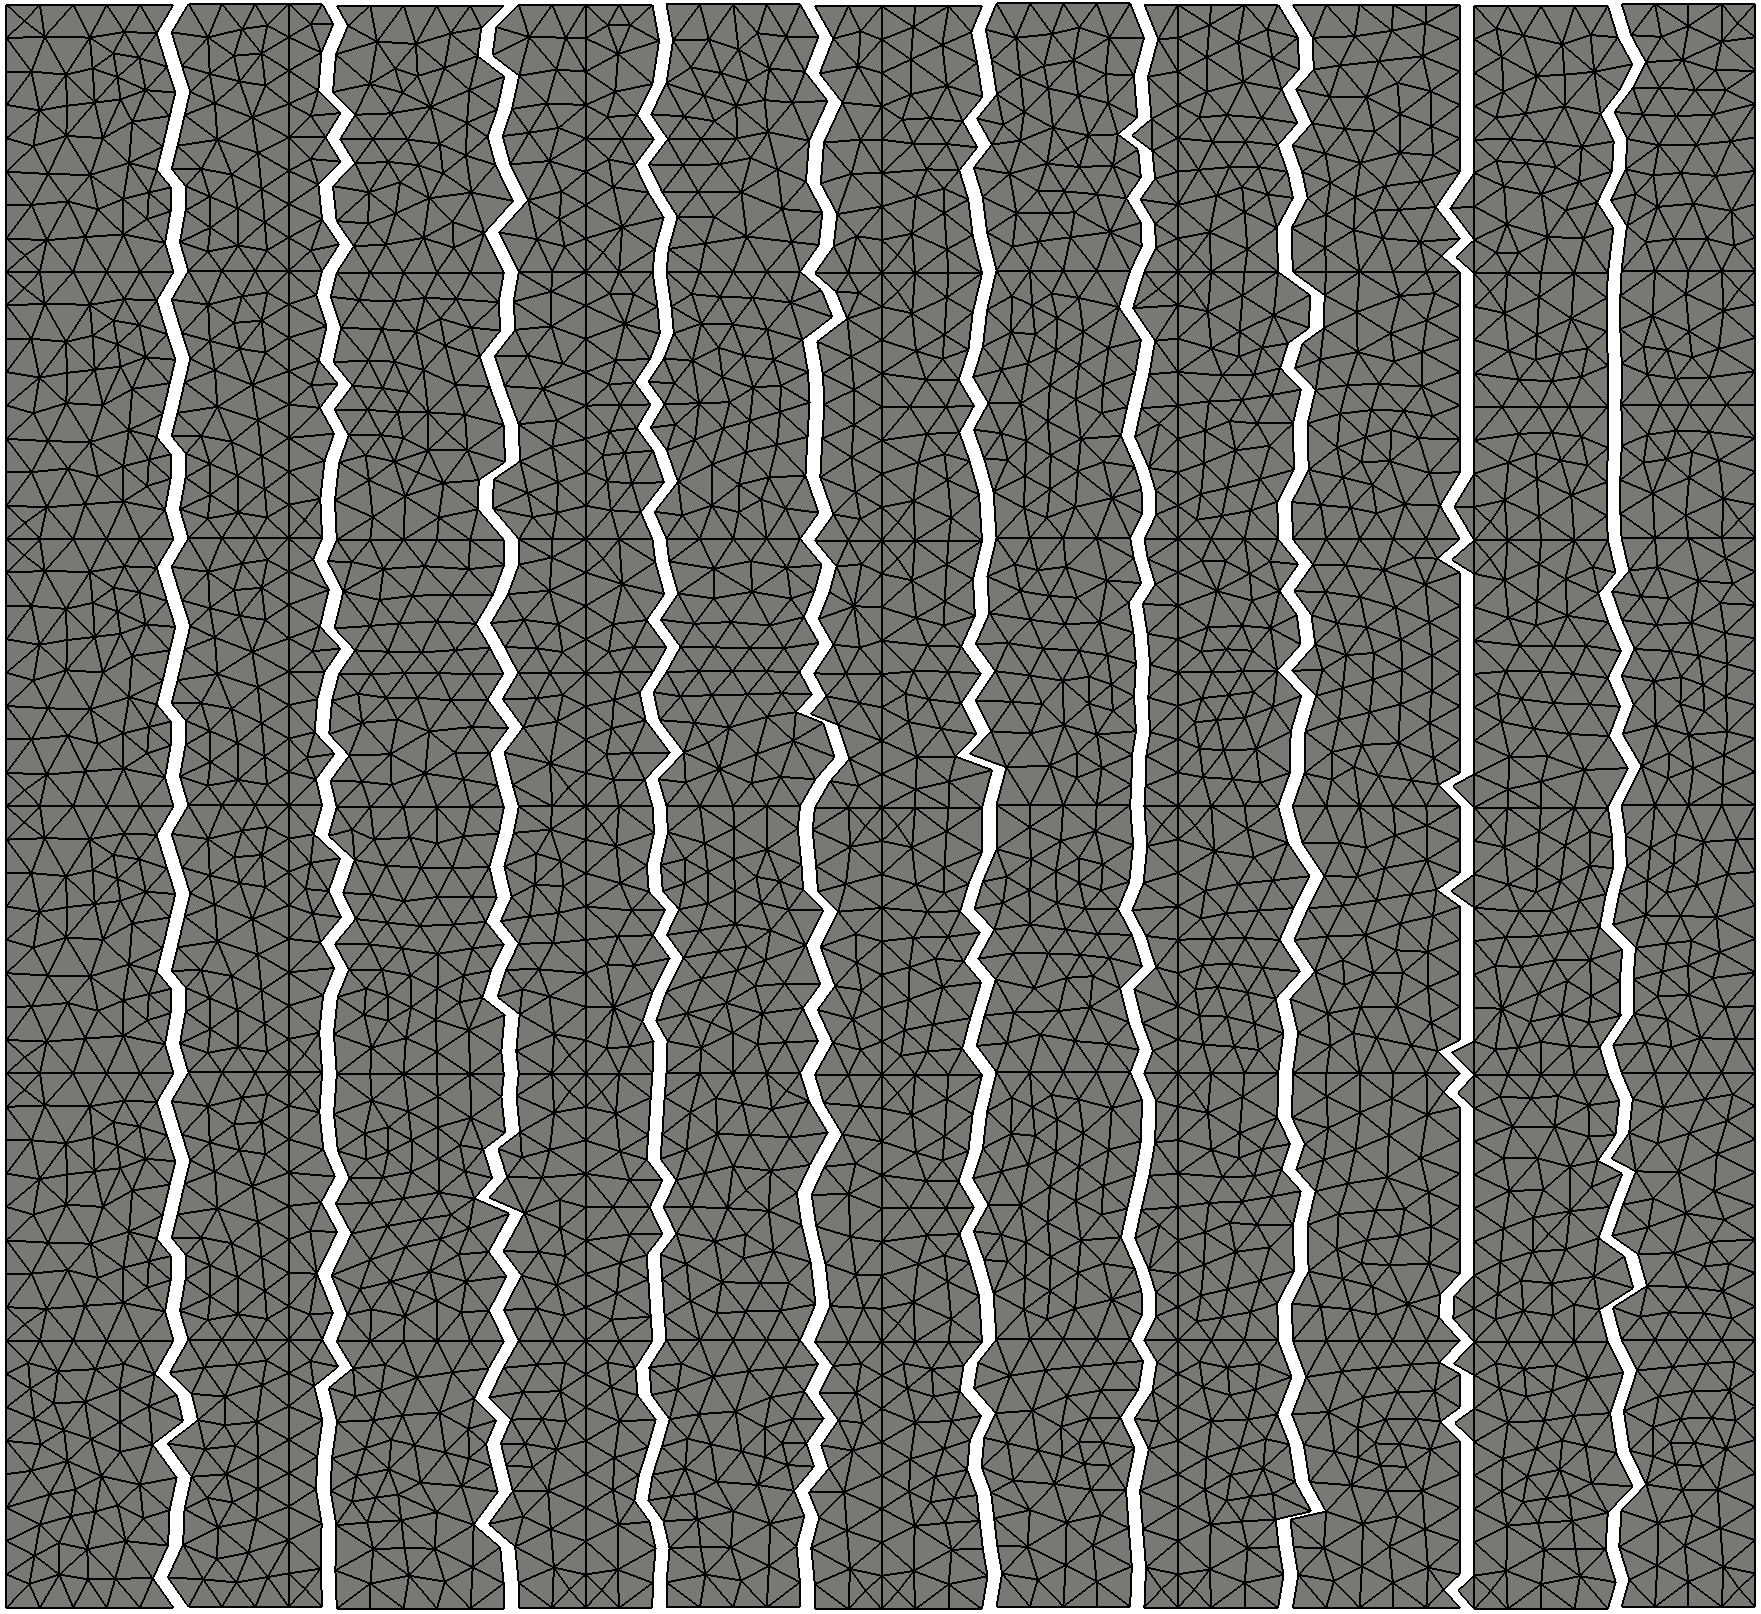
\includegraphics[width=\textwidth]{/home/lukas/Desktop/SA_Thesis/studies/2016-08-10_Partitioning/setup/chaco_11x1.png}
    \caption{vertical stripes}
  \end{subfigure}
  \hspace{1cm}
  \begin{subfigure}[b]{0.3\textwidth}
    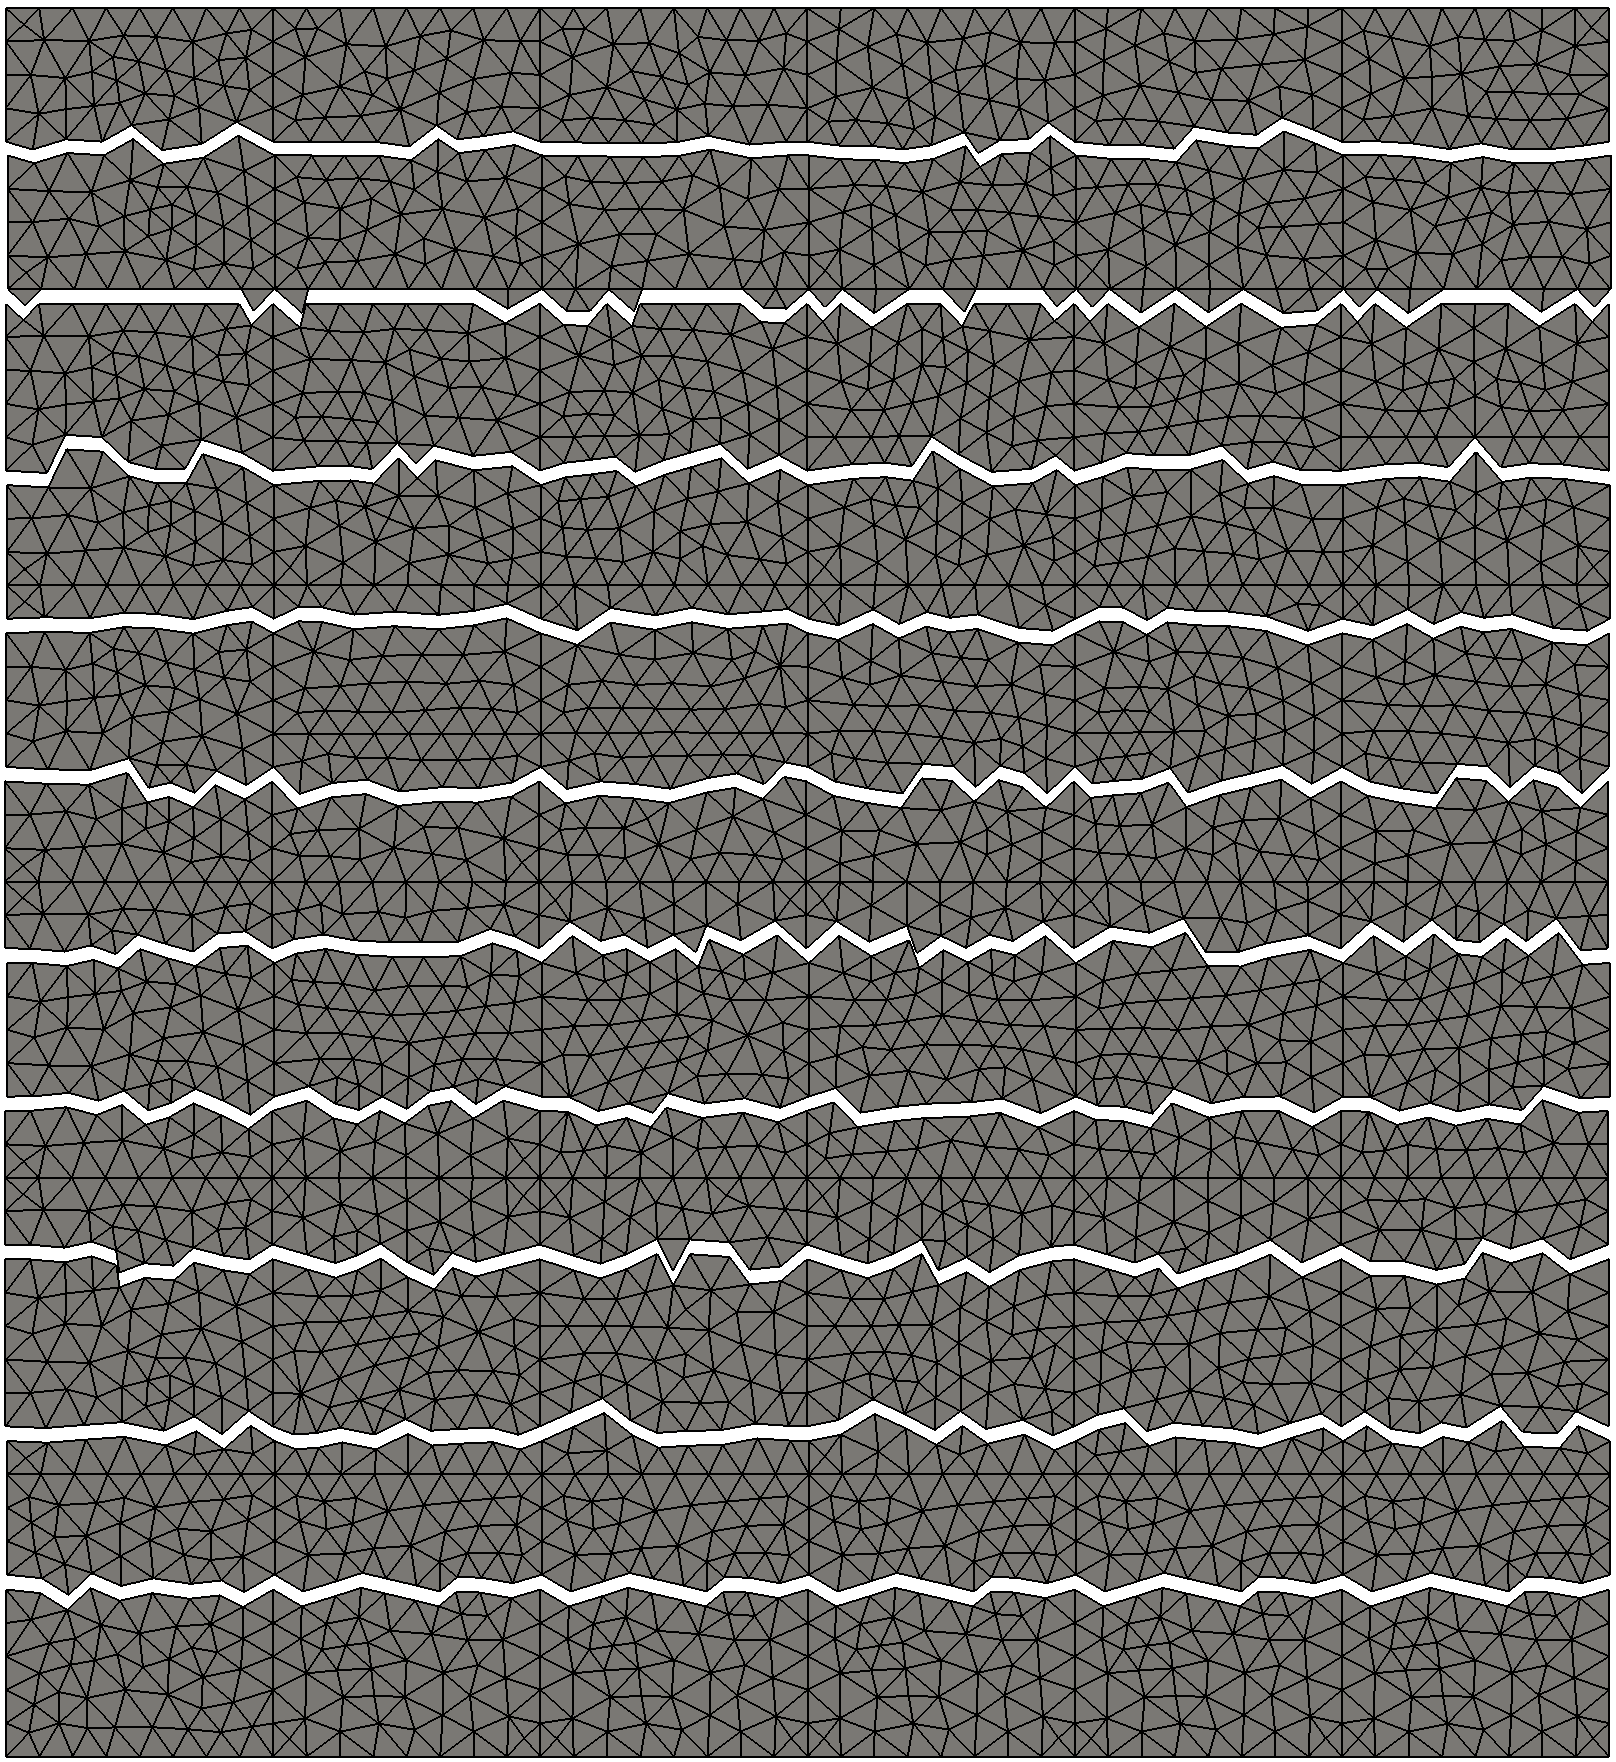
\includegraphics[width=\textwidth]{/home/lukas/Desktop/SA_Thesis/studies/2016-08-10_Partitioning/setup/chaco_1x11.png}
    \caption{horizontal stripes}
  \end{subfigure}
  \caption[Study of partitioning schemes: setup]{Different partitioning schemes. The top left example was manually partitioned into equally sized substructures keeping the number of interface unknowns low. The top right example was partitioned using chaco in GMSH. Finally, the bottom two examples were created using the Simple Partitioner Plug-in of GMSH. Here, the number of subdomains had to be drastically reduced, in order to get roughly the same size for the interface problem as in the top two examples. No material heterogenities were considered here. The results of this analysis are presented in Figure~\ref{fig:study_partitioning_numiter}}
  \label{fig:partitioning_schemes}
\end{figure} 


\begin{figure}[tb]
  \begin{center}
    %\fbox{\subimport{./}{./fig/tikz/study_inclusion.tex}}
    \includestandalone{./fig/tikz/study_partitioning_numiter}
    \caption[Study of partitioning schemes: \# iterations]{Results for the analysis of different partitioning schemes as described in Figure~\ref{fig:partitioning_schemes}. Firstly, we note that no dramatic difference between the regular partitioning and the automatic partitioning can be observed. Secondly, the stripe-like partitions performed far worse than the first two ones. Although less susceptible than the others, even the multi preconditioned schemes showed an increase of close to 100\% in that case. Event though, it was not possible to collect actual CPU-times, due to the Matlab implementation, taking into account, that the total number of substructures had to be significantly reduced for the stripe-like setups, it can be safely assumed that the advantage of reduced interconnectivity in the local stiffness matrices for stripe-like partitions does not justify choosing such a partitioning scheme.\\
      A comparison with regards to the number of search directions between the multi preconditioned algorithms for this example is provided in Figure~\ref{fig:study_partitioning_numsdir}. }
    \label{fig:study_partitioning_numiter}
  \end{center}
\end{figure}


\begin{figure}
  \begin{center}
    %\fbox{\subimport{./}{./fig/tikz/study_inclusion.tex}}
    \includestandalone{./fig/tikz/study_partitioning_residual}
    \caption[Study of partitioning schemes: residua]{Residual development for the partitioning scheme analysis described in Figure~\ref{fig:partitioning_schemes}. One can note that FETI-2 with a Geneo coarse grid shows good convergence rate for the first two partitioning schemes, whereas the FETI-2 convergence rate is significantly lower for stripe-like partitioning schemes. It shall be noted, that in the first to schemes, 6 Geneo modes were used per substructure, whereas the last two ones were calculated with 18 Geneo modes per substructure, so that the overall size of the coarse problem is the same for all four examples.}
    \label{fig:study_partitioning_residual}
  \end{center}
\end{figure}

\begin{figure}[tb]
  \begin{center}
    %\fbox{\subimport{./}{./fig/tikz/study_inclusion.tex}}
    \includestandalone{./fig/tikz/study_partitioning_numsdir}
    \caption[Study of partitioning schemes: \# search directions]{Results for the analysis of different partitioning schemes as described in Figure~\ref{fig:partitioning_schemes}. Particularly, this figure shows the number of chosen search directions for FETI-S and FETI-FAS. Although probably not optimal, the FETI-FAS algorithm is quite efficient in reducing the total number of search directions during the iterations. All four examples have been calculated with the default FETI-FAS parameters, as described in Section~\ref{sec:fetifas}. }
    \label{fig:study_partitioning_numsdir}
  \end{center}
\end{figure}


\section{Incompressibility}
Another well known problem for convergence is material incompressibility. The problem has been thoroughly analysed in ~\cite{Vereecke2003}.
In a linear elasticity, plane strain formulation, one can write
\begin{align}
  \tensor{\sigma}=\tensor{D}\tensor{\epsilon} = 2 \mu \tensor{\epsilon}+\lambda (tr(\epsilon)) \dmat{1} = \frac{E}{1+\nu} \tensor{\epsilon} + \frac{\nu E}{(1+\nu)(1-2 \nu)} tr(\tensor{\epsilon}) \dmat{1} 
\end{align}

Obviously, this term becomes problematic if $\nu \rightarrow 0.5$. In fact, the condition number of the stiffness matrix increases both with $\nu$ and with the model size. The problem has been analysed for the introduced FETI type of solvers. The setup is described in Figure~\ref{fig:setup_problem_incompressibility}. No material heterogenities were used here, in order to focus on incompressibility exclusively.

\begin{figure}[tb]
  \begin{center}
    \includegraphics[width=0.45\textwidth]{\studypath/2016-08-19_Incompresibility/setup/setup.pdf}~\hspace{0.5cm}
    \includegraphics[width=0.36\textwidth]{\studypath/2016-08-19_Incompresibility/setup/partitioning.pdf}~
    \caption[Study of incompressibility handling: setup]{Setup for the incompressibility analysis. The beam is divided into 24 substructures as shown in the right subfigure. Both the bottom and the top surface are clamped. A constant pressure is applied on the left side. The results for different Poission numbers are shown in Figure~\ref{fig:results_problem_incompressibility}}
    \label{fig:setup_problem_incompressibility}
  \end{center}
\end{figure}



\begin{figure}[tb]
  \begin{center}
    %\fbox{\subimport{./}{./fig/tikz/study_inclusion.tex}}
    \includestandalone{./fig/tikz/study_incompressibility}
    \caption[Study of incompressibility handling: \# iterations]{Results for the incompressibility analysis described in Figure~\ref{fig:results_problem_incompressibility}. Since incompressibility is only a problem in plane-strain calculations the same calculations with a plane-stress formulations are provided in the right figure. The figures clearly show, that the standard FETI-1 solver is very vulnerable in nearly incompressible simulations.}
    \label{fig:results_problem_incompressibility}
  \end{center}
\end{figure}

\begin{figure}%[tb]
  \begin{center}
    %\fbox{\subimport{./}{./fig/tikz/study_inclusion.tex}}
    \includestandalone{./fig/tikz/study_incompressibility_adaptive}
    \caption[Study of incompressibility handling: \# search directions]{Results for the incompressibility analysis described in Figure~\ref{fig:results_problem_incompressibility}. This figure shows the number of search directions used by the multi preconditioned schemes during the iterations. FETI-AS is not able to reduce search at all with the standard parameters here. FETI-AS does, but it tends to overshoot when approaching $\nu\rightarrow 0.5$. Overall, incompressibility seem to be a problem, where the adaptive schemes show no advantage compared to FETI-S}
    \label{fig:todo}
  \end{center}
\end{figure}

\FloatBarrier
\section{Inclusion}
The previous sections have indicated that parameter jumps along or across the interface pose a serious problem for DD-type of solvers.\\
One can however also create homogeneous interface examples, that still lead to highly increased iteration numbers. From an engineering point of view, this is due to substructures that show fundamentally different stiffness properties when considered separately than when considered in composite with the other substructures. The following considerations are inspired by~\cite{Gosselet2015}. The setup is briefly described in Figure~\ref{fig:setup_inclusion_problem} and the numerical results are presented in Figure~\ref{fig:results_inclusion_problem}.\\
The number of search directions used my the multi preconditioned solver is depicted in Figure~\ref{fig:results_inclusion_problem_adaptive}. Moreover, an visualization of the development of the residuum is provided in Figure~\ref{fig:results_inclusion_problem_residuum}.

\begin{figure}[tb]
  \begin{center}
    \includegraphics[width=0.4\textwidth]{\studypath/2016-08-19_Inclusion/setup/setup.pdf}~
    \hspace{1cm}~
    \includegraphics[width=0.35\textwidth]{\studypath/2016-08-19_Inclusion/setup/partitioning.pdf}
    \caption[Study of inclusion handling: setup]{Setup for the inclusion analysis. The left figure shows the material distribution. The right figure depicts the partitioning into substructures. As shown, every substructure consists of a lattice around the substructure border and another material within (inclusion). An setup like this as coefficient jumps neighter along nor across the interface. Nevertheless FETI-solver are challenged by it. Figure~\ref{fig:results_inclusion_problem} shows the iteration counts for the different FETI-algorithms}
    \label{fig:setup_inclusion_problem}
  \end{center}
\end{figure}	

\begin{figure}[tb]
  \begin{center}
    %\fbox{\subimport{./}{./fig/tikz/study_inclusion.tex}}
    \includestandalone{./fig/tikz/study_inclusion}
    \caption[Study of inclusion handling: \# iterations]{Results for the inclusion problems as described in Figure~\ref{fig:setup_inclusion_problem}. The top two figures show the calculations with the default lumped preconditioner, the bottom ones with a full Dirichlet preconditioner(see Section~\ref{sec:precond}. The left figures were calculated with inclusion to substructure ration of $\frac{L_{inclusion}}{L_{substructure}}=0.9$, the right figures with $\frac{L_{inclusion}}{L_{substructure}}=0.95$.  The graphs show that FETI-S and FETI-2(Geneo) show less sever increases in the iteration numbers than FETI-1, when the stiffness ratio $\frac{E_{inclusion}}{E_{lattice}}$ is decreased. As expected, the problematic case is the one with soft inclusions inside a stiff lattice. In that case, the solver drastically underestimates the deformation. The overestimation of deformation for the contrary case is not critical. What is more, one can also notice that FETI-2 is obviously not able to correctly detect the bad modes, when a lumped preconditioner is used. This is intuitive when looking at the very definition of the two preconditioner types in Equations~\eqref{eq:precond}\eqref{eq:precond_mscaled}\eqref{eq:precond_kscaled}. Since the lumped preconditioner neglects the Inner stiffness components $\stiffmat_{ii}$, no information abut the inner stiffness change enters the Geneo algorithms.}
    \label{fig:results_inclusion_problem}
  \end{center}
\end{figure}

\begin{figure}[tb]
  \begin{center}
    \subimport{./}{./fig/tikz/study_inclusion_residual}
    \caption[Study of inclusion handling: residua]{Residuum development for the inclusion analysis with lumped and Dirichlet preconditioners and soft as well as stiff inclusions. The case of hard inclusions obviously does not pose any problems. As mentioned in Figure~\ref{fig:results_inclusion_problem} the top two figures again confirm, that Geneo can only play out its advantages in terms of convergence rate, when the Dirichlet preconditioner is used. Otherwise it is not able to detect soft inclusions. However, the Dirichlet preconditioner comes with a significantly increased price, as outlined in Section~\ref{sec:precond}. }
    \label{fig:results_inclusion_problem_residuum}
  \end{center}
\end{figure}


\begin{figure}[tb]
  \begin{center}
    \subimport{./}{./fig/tikz/study_inclusion_adaptive}
    %\includestandalone{./fig/tikz/study_inclusion_adaptive}
    \caption[Study of inclusion handling: \# search directions with lumped preconditioner]{Results for the inclusion problems as described in Figure~\ref{fig:setup_inclusion_problem} with a lumped preconditioner. This plots compare the number of search directions used during the iterations of the FETI-S and the FETI-FAS algorithm. For the top two figures, the FETI-FAS algorithms shows mediocre results.For the bottom figure, FETI-FAS successfully detects the expandability of almost all search directions ans thereby reduced the computational effort significantly. The application of FETI-FAS did not pose any problems here, since the standard parameters as introduces in Section~\ref{sec:default_parameters} were used. }
    \label{fig:results_inclusion_problem_adaptive}
  \end{center}
\end{figure}

\begin{figure}[tb]
  \begin{center}
    \subimport{./}{./fig/tikz/study_inclusion_adaptive_dirich}
    %\includestandalone{./fig/tikz/study_inclusion_adaptive}
    \caption[Study of inclusion handling: \# search directions with Dirichlet preconditioner]{Results for the inclusion problems as described in Figure~\ref{fig:setup_inclusion_problem} wit a Dirichlet Preconditioner. This plots compare the number of search directions used during the iterations of the FETI-S and the FETI-FAS algorithm. When compared to Figure~\ref{fig:results_inclusion_problem_adaptive}, we note that the appropriate choice of the contraction factor $\tau$ is obviously, among others, dependent on the preconditioner type used, while FETI-FAS  performs reasonably well for both cases.}
    \label{fig:results_inclusion_problem_adaptive_dirich}
  \end{center}
\end{figure}



\chapter{Summary}\label{cha:summary}

In conclusion, the FETI-method has been introduced as a prominent domain decomposition method for structural mechanics problems. The underlying motivation for domain decomposition methods has been described in Chapter~\ref{cha:introduction} and a quick comparison to other DD methods has been drawn.\\
Chapter~\ref{cha:feti_formulation} introduced the standard FETI method(FETI-1), as first described by \cite{Farhat1991} and derived all relevant equations. It has then been shown, that the FETI-1 method shows some severe deficiencies, especially for the problems mentioned in Chapter~\ref{cha:numerical_assesment}.\\
Variations of the FETI-1 method, namely FETI-2 and FETI-S have therefore been described in Chapter~\ref{cha:feti_solvers} and their theoretical potentials have been discussed.
Inspired by\cite{Spillane2016} the concept of an Adaptive Multi Preconditioned Conjugate Gradient algorithm has then been adapted to the FETI-method leading to the FETI-A algorithm. To my knowledge this has not been done before.\\
Since the FETI-AS algorithm depends on a user specified threshold $\tau$ which is delicate to choose, a variation of the algorithm, the Fast Adaptive Simultaneous FETI solver(FETI-FAS) has been proposed in Section~\ref{sec:fetias}.\\
All five algorithms have been thoroughly discussed and summarized in Chapter~\ref{cha:feti_solvers}.\\
Chapter~\ref{cha:numerical_assesment} has then been dedicated to an intensive analysis and comparison of the five described FETI-algorithms. For that purpose four setups, covering the most challenging situations for DD methods, have been devised and solved with each algorithm. Several conclusions have been drawn.\\
First of all, the before mentioned inferiority of the FETI-1 method has been confirmed in each setup. Moreover, it has been shown, that FETI-S and FETI-2(Geneo) show comparable results, with slight advantages for the FETI-S(Geneo) approach when it comes to the total iteration number. However, as described in Chapter~\ref{cha:feti_solvers} the Geneo approach involves the solution of eigenvalue problems on the substructure interfaces. The overall conclusion therefore was, that the slightly reduced iteration count of the Geneo approach, does not justify the large computational overhead as compared to the FETI-S algorithm, especially with the efficient implementation as outlined in Section~\ref{sec:fetis}.\\
Moreover, the examples generally confirmed that one usually can neglect a large part of the search directions in the FETI-S solver, and still get reasonable iteration numbers. This was the main idea behind the Adaptive Simultaneous FETI solvers. It has also been shown that the choice of an appropriate parameter $\tau$ in the FETI-AS algorithm is a delicate issue. While prescribing a desired contraction factor, instead of directly prescribing $\tau$ mediated the problem, a general recommendation for $\tau$ can still not be drawn.\\
Our simulations thus suggested that the FETI-FAS solver can be favoured as a more reasonable, easier to choice that performs very well in most cases.\\
\\
For the purpose of this thesis, an object oriented finite element code (FEMAC) has been written in Matlab\cite{FEMAC}.
\chapter{Outlook}

The potentials of the FETI-As approaches have been vividly demonstrated in Chapter~\ref{cha:numerical_assesment}.\\
Subsequent research should thus be focused on the development of the Simultaneous FETI  methods. When it comes to FETI-AS, a closer look can be paid upon the appropriate choice of $\tau$. It seems reasonable that better rules can be derived.\\
WE also propose to focus on the herein newly introduced FETI-FAS method. The solver parameters can definitely still be tuned, and an application to dynamic problems remains to be done.\\
This paper focused on a simple small strain, linear finite element formulation. As a first step, the method should thus be generalized to a non-linear, dynamic formulation.\\
Since the herein used code was written in Matlab, meaningful CPU-time analyses could not have been carried out and thus remain to be done too.\\
Special attention should also be given to an profound analyses of the parallel scalability of the method.\\
Further analyses should be carried out on an efficient low-level implementation like C++ or FORTRAN.

%\pagepreak
\backmatter
\AMPrintBibliography
%\bibliographystyle{plain}

\end{document}
